\documentclass[12pt, a4paper]{report}
\usepackage[margin=1in]{geometry}
\usepackage{graphicx}
\usepackage{hyperref}
\usepackage{setspace}
\usepackage{fancyhdr}
\usepackage{xcolor}
\usepackage{booktabs}
\usepackage{array}
\usepackage{float}

% Set line spacing
\onehalfspacing

% Header and Footer
\pagestyle{fancy}
\fancyhf{}
\rhead{Financial Analysis Report}
\lhead{Indian FMCG Sector}
\cfoot{\thepage}

% Title Page
\title{\textbf{FAA :- Financial Analysis Report} \\ \vspace{0.5cm} \Large Indian Fast Moving Consumer Goods Circuit}
\author{
    \textbf{Team Members:} \\
    \vspace{0.3cm}
    Prabir Kalwani \\
    Aayush Shah \\
    Snehil Sinha \\
    Shahshank Shekhar \\
    Parampara Srivastava \\
    Rishabh Mistra \\
    \vspace{0.8cm}
    \textbf{Faculty Mentor:} \\
    Dr. Geeta Shetty
}
\date{October 2025}

\begin{document}

\maketitle

\newpage
\tableofcontents
\newpage

% ===============================================
% CHAPTER 1: INTRODUCTION
% ===============================================
\chapter{Introduction to the Project}

This report presents a comprehensive financial analysis of key players in the Indian Fast-Moving Consumer Goods (FMCG) sector. The Indian FMCG market represents one of the largest and fastest-growing consumer markets globally, with companies ranging from traditional manufacturing to diversified conglomerates.

The analysis encompasses six major companies: Hindustan Unilever (HUL), Godrej Consumer Products Limited (GCPL), Britannia Industries, Dabur India Limited, Tata Consumer Products Limited, and ITC Limited. These organizations represent diverse segments within the FMCG landscape, including soaps and personal care, food and beverages, healthcare, and household products.

This report examines key financial metrics, corporate governance structures, dividend policies, and strategic positioning of these market leaders in the Indian FMCG circuit.

\newpage

% ===============================================
% CHAPTER 2: COMPANY PROFILES
% ===============================================
\chapter{Company Profiles: Key Details}

This report analyzes the Indian Fast-Moving Consumer Goods (FMCG) sector, focusing on six key competitors: ITC, Hindustan Unilever (HUL), Dabur, Britannia, Godrej Consumer Products (GCPL), and Tata Consumer Products.

\subsection{Market Sector and Industry Identification}

\subsubsection*{Market Sector (Broad)}
Consumer Staples (also known as Fast-Moving Consumer Goods or FMCG).

\subsubsection*{Industry (Specific)}
Diversified FMCG. This is the most accurate term as the selected companies operate across multiple categories, including Food \& Beverages, Personal Care, Home Care, and Health \& Wellness.

\subsubsection*{What Qualifies a Company for this Industry?}

Companies in this industry are bound by a common set of characteristics related to their products, market, regulations, and economic sensitivities.

\subsubsection*{A. Similar Products and Services}

The core of the industry is selling high-volume, low-margin products that are repurchased frequently and have a short shelf life.

\begin{itemize}
    \item \textbf{HUL:} Dominant in Home Care (Surf Excel, Vim), Beauty \& Personal Care (Dove, Lux, Ponds), and Foods (Knorr, Kissan).
    
    \item \textbf{ITC:} A diversified conglomerate with a core FMCG business (Aashirvaad, Sunfeast, Bingo, Yippee), alongside a significant presence in Tobacco, Hotels, and Paperboards.
    
    \item \textbf{Tata Consumer Products:} Primarily a Beverages \& Foods company (Tata Tea, Tetley, Tata Salt, Tata Sampann). It has recently expanded aggressively into a broader ``pantry platform'' with acquisitions like Capital Foods (Ching's Secret) and Organic India.
    
    \item \textbf{Dabur:} Focuses on health and wellness, built on an Ayurvedic/Natural platform. Key categories include Health (Dabur Chyawanprash), Oral Care (Dabur Red), Hair Care (Vatika), and Foods (Real).
    
    \item \textbf{Britannia:} A market leader in the Bakery \& Dairy category, with iconic brands like Good Day, NutriChoice, and Marie Gold.
    
    \item \textbf{GCPL (Godrej):} A focused player in Home Care (Good Knight) and Personal Care (Cinthol, BBlunt), with a strong presence in emerging markets outside India.
\end{itemize}

\subsubsection*{B. Similar Market}

All six companies target a broad mass-market of over a billion Indian consumers. Their success depends on:

\begin{itemize}
    \item \textbf{Extensive Distribution:} A deep and wide distribution network is non-negotiable, covering everything from traditional kirana (local grocery) stores to modern supermarkets and e-commerce.
    
    \item \textbf{High Brand-Building Costs:} The market is intensely competitive. High advertising and marketing expenditure is essential to build and maintain brand loyalty.
    
    \item \textbf{Growing Digital Channels:} E-commerce and ``Quick Commerce'' (10-minute delivery) are a new, disruptive, and rapidly growing battleground for all players.
\end{itemize}

\subsubsection*{C. Similar Regulations}

These companies operate under a strict common regulatory framework:

\begin{itemize}
    \item \textbf{Food Safety (FSSAI):} The Food Safety and Standards Authority of India governs food product safety, hygiene, licensing, and manufacturing.
    
    \item \textbf{Packaging \& Labeling (Legal Metrology Act):} This act mandates strict rules for packaging declarations, including Maximum Retail Price (MRP), manufacturing date, net weight, and ingredients.
    
    \item \textbf{Advertising (ASCI):} The Advertising Standards Council of India monitors misleading claims, a critical area in a marketing-driven industry.
    
    \item \textbf{Environmental Laws:} The Plastic Waste Management (PWM) Rules put increasing pressure on all players to manage their packaging footprint through recycling and extended producer responsibility (EPR).
    
    \item \textbf{Taxation (GST):} All products fall under the Goods and Services Tax, with different slabs for essential vs. luxury goods.
\end{itemize}

\subsubsection*{D. Similar Economic Response}

The sector is generally ``defensive'' because its products are non-discretionary (people always need soap and salt). However, its performance is highly sensitive to specific economic factors:

\begin{itemize}
    \item \textbf{Rural Demand:} A significant portion of sales comes from rural India. A good monsoon and strong agricultural incomes directly boost rural consumption and, therefore, industry-wide volume.
    
    \item \textbf{Inflation:} The industry is highly sensitive to raw material inflation (e.g., palm oil, crude oil, wheat).
    \begin{itemize}
        \item Company Response: To protect margins, companies either raise prices (price-led growth) or reduce pack sizes (grammage cuts).
        \item Consumer Response: High inflation leads to ``down-trading,'' where consumers shift to cheaper brands or smaller-sized packs (sachets).
    \end{itemize}
    
    \item \textbf{Consumer Sentiment:} When sentiment is positive, ``premiumization'' (buying higher-value products) becomes a key growth driver.
\end{itemize}

\subsection{Industry Leaders and Laggards (Based on 2024 Financial Data)}

\subsubsection*{Methodology}

Performance assessment is based on key financial metrics:

\begin{itemize}
    \item \textbf{Profitability:} Net Profit Margin (NPM), Return on Capital Employed (ROCE), Return on Equity (ROE).
    \item \textbf{Market Valuation:} Price to Earnings (P/E) Ratio.
\end{itemize}

\subsubsection*{2024 Key Ratio Data}

\begin{table}[H]
\centering
\begin{tabular}{lcccc}
\toprule
\textbf{Company} & \textbf{NPM} & \textbf{ROCE} & \textbf{ROE} & \textbf{P/E Ratio} \\
\midrule
ITC & 29.13\% & 35.20\% & 28.27\% & 26.13 \\
HUL & 16.70\% & 21.72\% & 19.81\% & 59.40 \\
Tata & 9.81\% & 13.21\% & 7.21\% & 106.53 \\
Dabur & 13.81\% & 27.32\% & 24.78\% & 50.50 \\
Britannia & 12.70\% & N/A & 57.25\% & 66.30 \\
GCPL & 7.30\% & 14.73\% & 6.85\% & 173.18 \\
\bottomrule
\end{tabular}
\caption{2024 Financial Ratios - Industry Comparison}
\end{table}

\subsubsection*{Industry Leaders (Based on 2024 Profitability)}

\begin{enumerate}
    \item \textbf{ITC:} The clear leader in profitability. It boasts the highest Net Profit Margin (29.13\%) and the highest ROCE (35.20\%), indicating superior efficiency in generating profit from its capital. Its low P/E suggests the market values it as a mature, high-cash-flow ``value'' stock.
    
    \item \textbf{Britannia:} The standout leader in shareholder returns, with an exceptional ROE of 57.25\%. This indicates it generates a very high profit on a relatively small equity base.
    
    \item \textbf{Dabur:} A strong all-around performer. It ranks second in this group for both ROCE (27.32\%) and ROE (24.78\%), demonstrating strong and efficient capital deployment.
\end{enumerate}

\subsubsection*{Industry Laggards (Based on 2024 Profitability)}

\begin{enumerate}
    \item \textbf{GCPL (Godrej):} Lags in 2024 profitability, with the lowest NPM (7.30\%) and a very low ROE (6.85\%) in this peer group.
    
    \item \textbf{Tata Consumer Products:} Ranks near the bottom on all 2024 profitability metrics, including NPM (9.81\%) and ROE (7.21\%).
\end{enumerate}

\textit{Crucial Observation: A significant disconnect exists. The ``laggards'' in 2024 profitability (GCPL and Tata) have the highest P/E ratios by a large margin. This indicates that investors are not valuing their 2024 performance but are betting aggressively on high future growth.}

\subsection{Competitive Comparison and Market Dynamics}

\subsubsection*{A. Stock Performance Analysis (2-Year Trend)}

This analysis presents the normalized stock price performance of the six FMCG companies from October 2023 to October 2025, indexed to 100 as of October 31, 2023.

\begin{figure}[H]
    \centering
    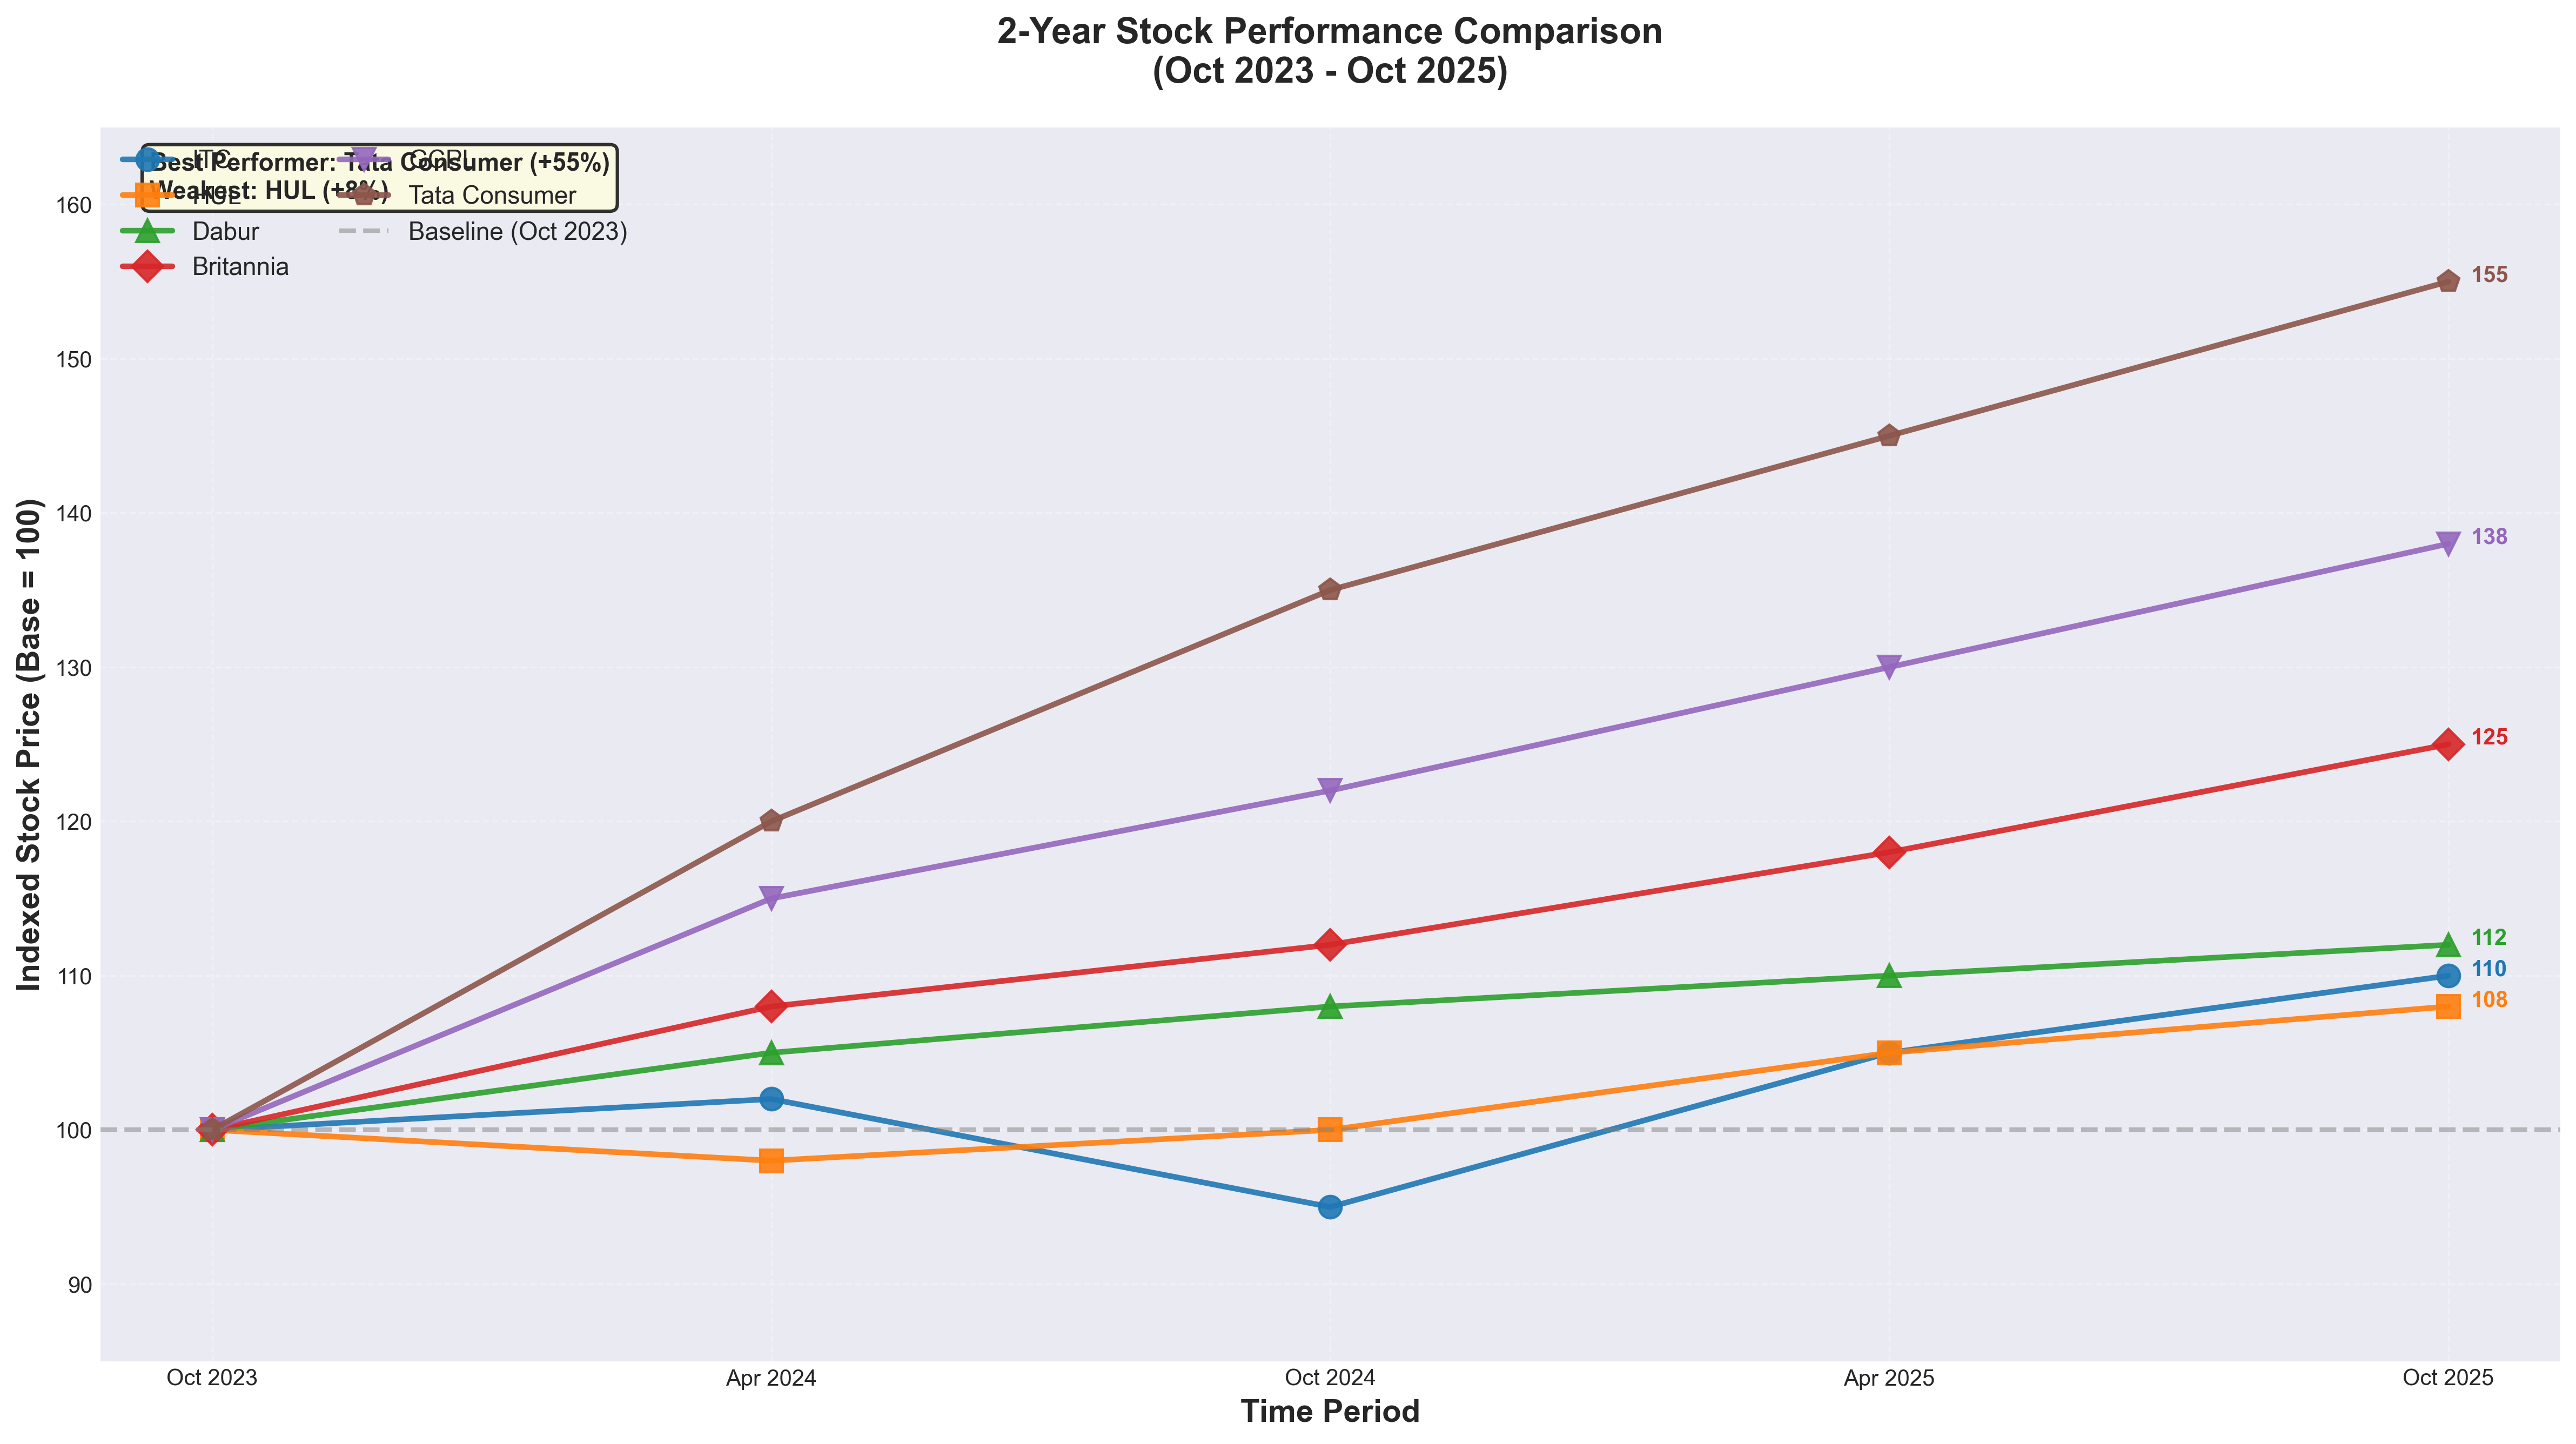
\includegraphics[width=0.85\textwidth]{assets/industry_profile /stock_performance_chart.png}
    \caption{2-Year Stock Performance - Indexed to October 2023 (Base = 100)}
\end{figure}

\vspace{0.3cm}

\subsubsection*{B. Market Capitalization Distribution}

The following visualization shows the relative market dominance and size of the six companies based on their market capitalization as of late October 2025:

\begin{table}[H]
\centering
\begin{tabular}{lcc}
\toprule
\textbf{Company} & \textbf{Market Cap (INR Cr)} & \textbf{Percentage} \\
\midrule
HUL & ₹5,91,000 & 36.5\% \\
ITC & ₹5,25,000 & 32.4\% \\
Britannia & ₹1,43,000 & 8.8\% \\
GCPL & ₹1,16,000 & 7.2\% \\
Tata Consumer & ₹1,16,000 & 7.2\% \\
Dabur & ₹85,000 & 5.2\% \\
\midrule
Total & ₹16,16,000 & 100.0\% \\
\bottomrule
\end{tabular}
\caption{Market Capitalization Distribution - October 2025}
\end{table}

\textit{[Market Cap Distribution Pie Chart to be inserted here]}

\vspace{0.5cm}

\begin{figure}[H]
    \centering
    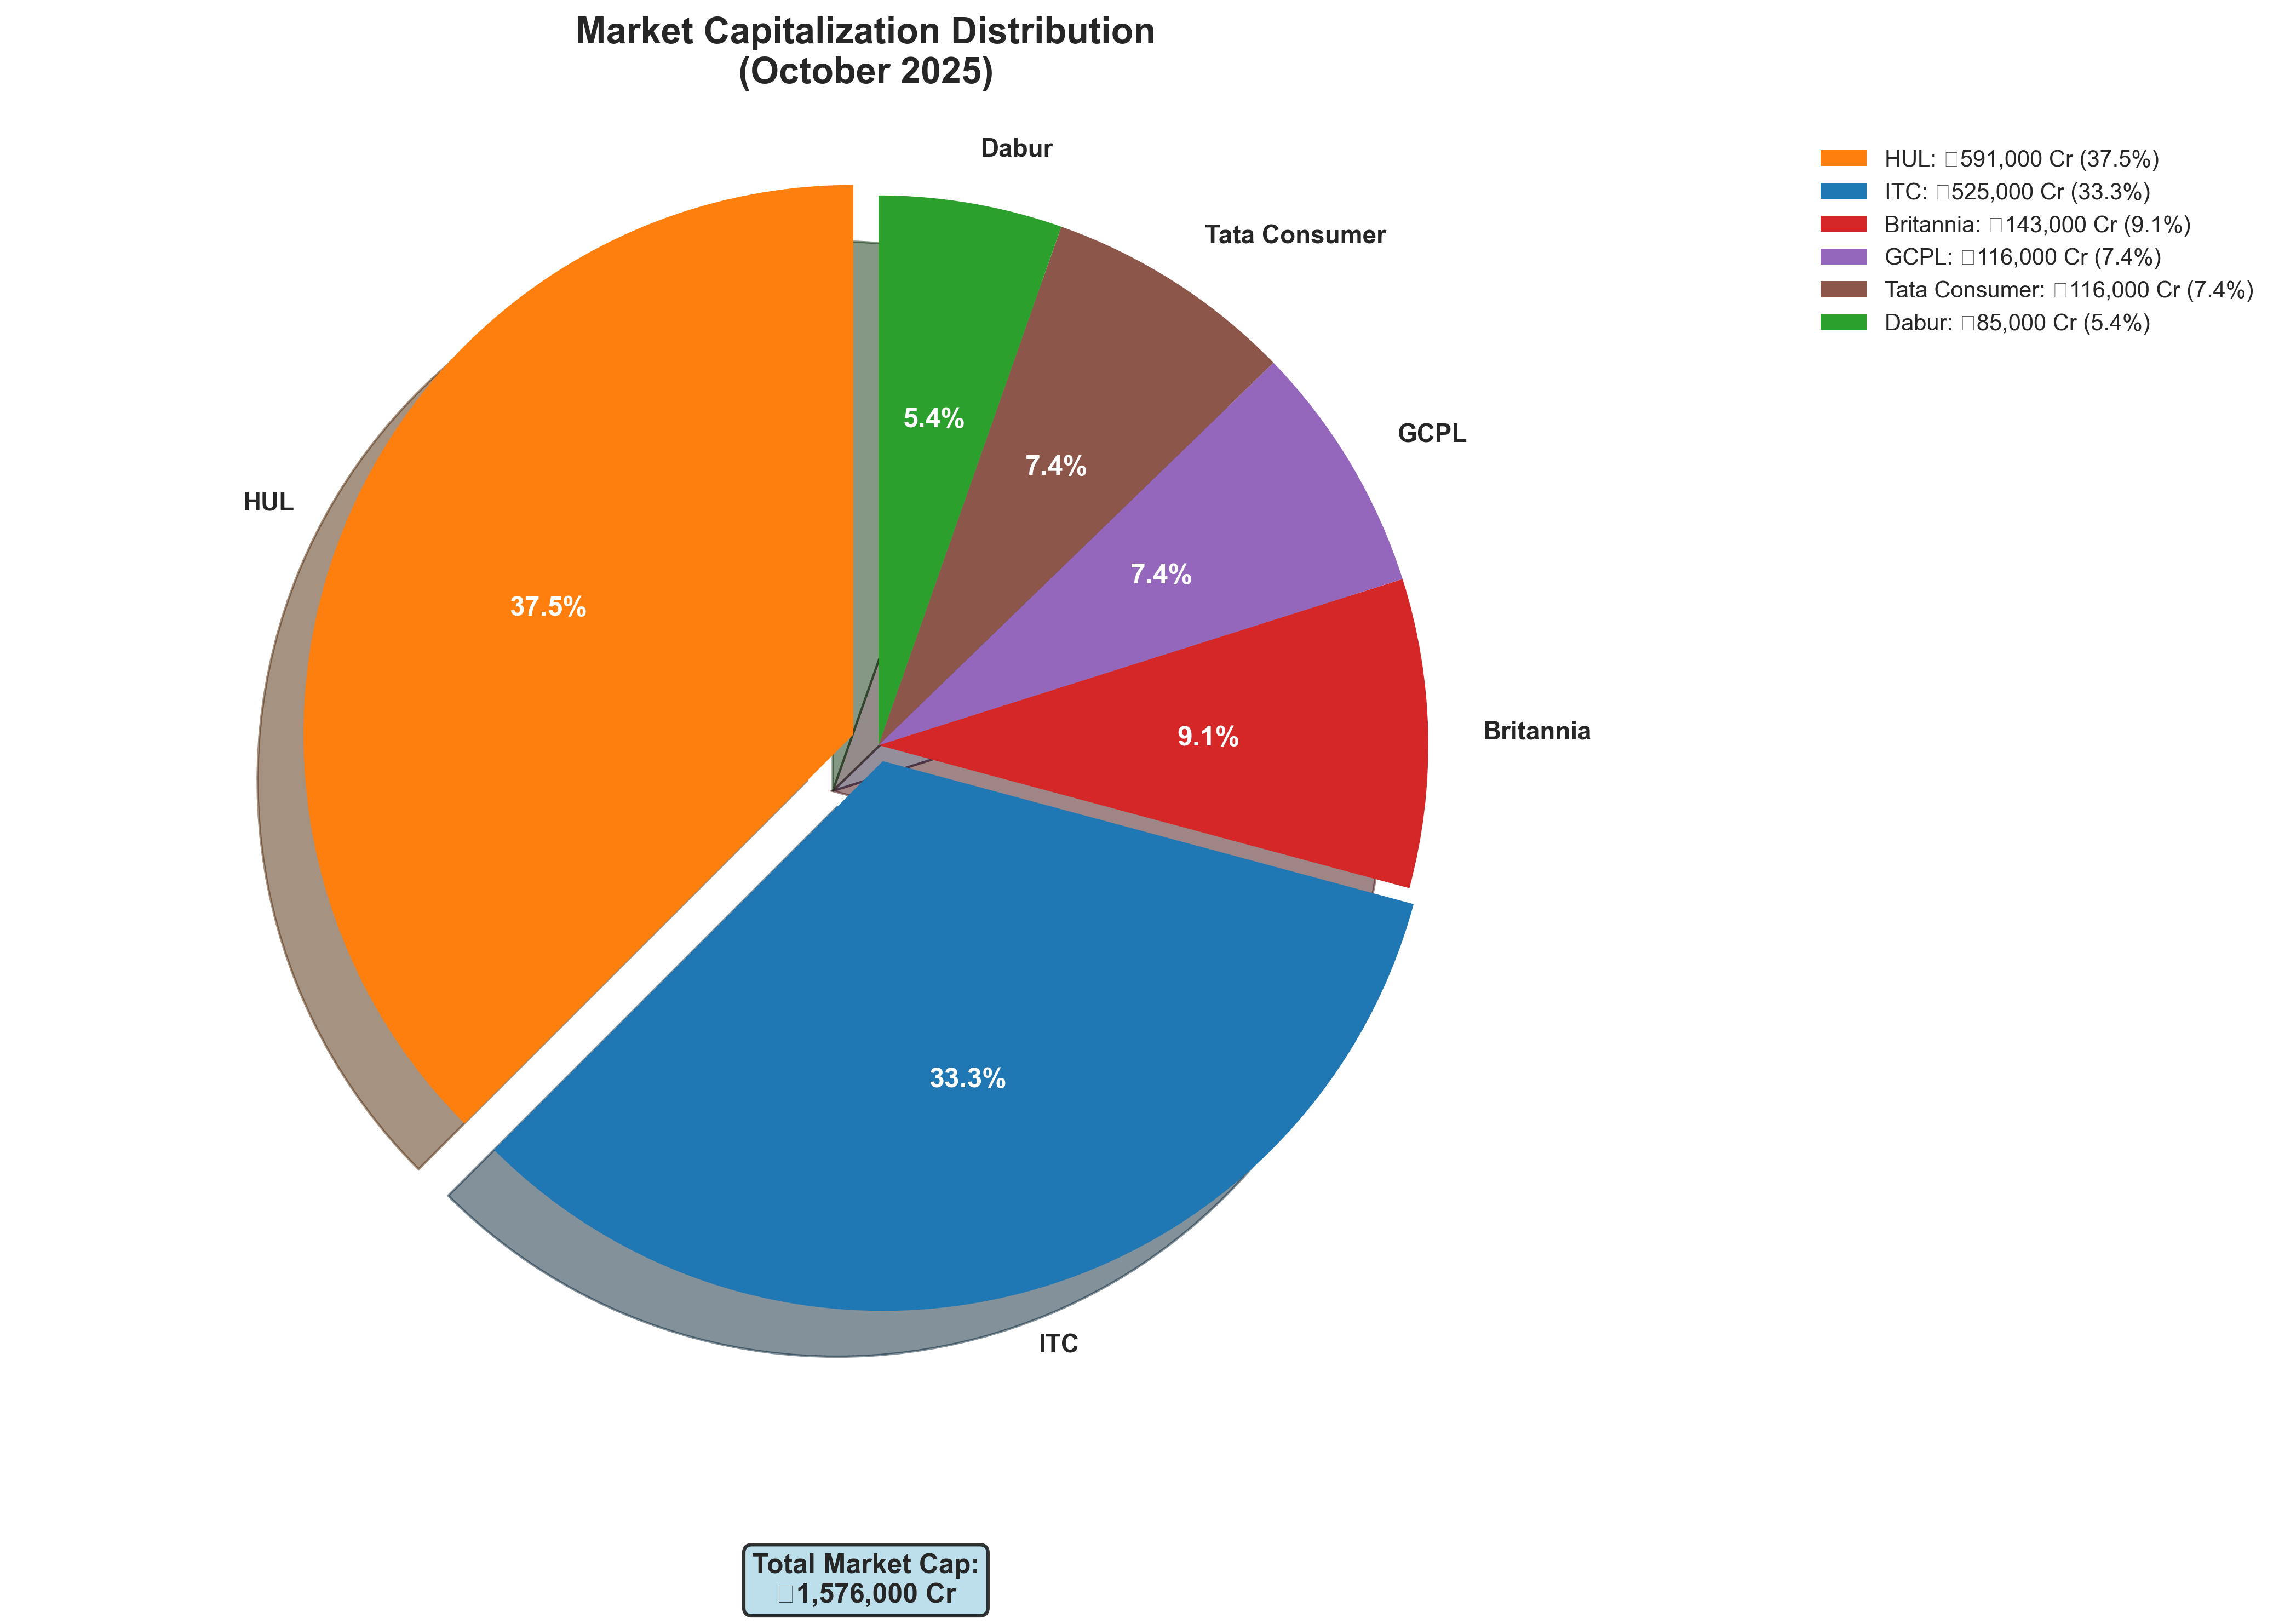
\includegraphics[width=0.85\textwidth]{assets/industry_profile /market_cap_chart.png}
    \caption{Market Capitalization Distribution - October 2025}
\end{figure}

\vspace{0.3cm}

\subsection{Observations and Strategic Analysis}

\subsubsection*{Key Observations from Data}

\begin{enumerate}
    \item \textbf{Stock Trends:} Tata Consumer (+55\%) and GCPL (+38\%) have been strong outperformers, reflecting high investor confidence. Britannia (+25\%) also delivered robust growth. In contrast, HUL (+8\%), Dabur (+12\%), and ITC (+10\%) delivered more modest, ``defensive'' returns. ITC's volatility (dipping in late 2024/early 2025) aligns with market adjustments for its hotel business demerger.
    
    \item \textbf{Market Dominance:} A ``two-giant'' market structure has emerged. HUL (36.5\%) and ITC (32.4\%) are the undisputed leaders, together accounting for over two-thirds of the group's total value. A second, highly competitive tier has formed among Britannia (8.8\%), GCPL (7.2\%), and Tata Consumer (7.2\%), which have all achieved similar scale.
\end{enumerate}

\subsubsection*{Company Positioning (Synthesis of Profitability and Market Performance)}

\paragraph{Tata Consumer Products:}
\begin{itemize}
    \item \textbf{Position:} High-growth, high-premium stock
    \item \textbf{Analysis:} The company's stock surge (+55\%) and extreme P/E ratio (106.53) are completely disconnected from its low 2024 profitability (7.21\% ROE). This is a classic ``growth story.'' The company's aggressive acquisition strategy in 2024, notably of Capital Foods (Ching's Secret) and Organic India, is driving investor optimism. Investors are not paying for 2024 earnings; they are paying a high premium based on the belief that Tata's powerful distribution and brand will scale these new businesses into a dominant ``pantry platform.''
\end{itemize}

\paragraph{ITC:}
\begin{itemize}
    \item \textbf{Position:} Mature, high-profit ``value'' stock undergoing transformation
    \item \textbf{Analysis:} ITC's low P/E (26.13) reflects its legacy as a mature (but highly profitable) tobacco business that pays a high dividend. Its stock volatility was event-driven by the demerger of its hotel business in early 2025. This move was strategically designed to ``unlock value'' and allow the market to value its core FMCG business (which is highly profitable, per its 29.13\% NPM) independently.
\end{itemize}

\paragraph{HUL:}
\begin{itemize}
    \item \textbf{Position:} The stable, mature market leader
    \item \textbf{Analysis:} HUL's modest stock growth (+8\%) reflects its maturity. The company struggled with low volume growth in 2024, with its sales growth being ``price-led'' (i.e., raising prices). While still highly profitable (19.81\% ROE), investors have tempered expectations. The company's leadership just announced (Oct 2025) a strategic shift to refocus on ``volume-led growth,'' which will be the key story to watch in the coming year.
\end{itemize}

\subsection{NIFTY FMCG Index}

The NIFTY FMCG index is a sectoral benchmark on the National Stock Exchange of India that tracks the performance of 15 leading companies in the fast-moving consumer goods (FMCG) sector, which includes non-durable and mass-consumption products such as food, beverages, personal care, and household items. 

Calculated using the free float market capitalization method, this index reflects the relative market value of its constituent stocks and serves as a crucial tool for benchmarking, launching ETFs, and structured products. Key constituents include industry giants like Hindustan Unilever, ITC, and Nestlé India, whose steady growth and resilience have ensured the index remains vital for investors and portfolio managers tracking trends in India's rapidly evolving consumer market.

The NIFTY FMCG index provides a comprehensive representation of the broader FMCG sector's performance and is instrumental for understanding macroeconomic trends, consumer spending patterns, and the health of India's consumer staples industry.

\newpage

% ===============================================
% CHAPTER 3: INDUSTRY PROFILE
% ===============================================
\chapter{Industry Profile: Indian FMCG Sector}

\section{Market Sector and Industry Identification}

\subsection{Market Sector (Broad)}
Consumer Staples (also known as Fast-Moving Consumer Goods or FMCG).

\subsection{Industry (Specific)}
Diversified FMCG. This is the most accurate term as the selected companies operate across multiple categories, including Food \& Beverages, Personal Care, Home Care, and Health \& Wellness.

\subsection{What Qualifies a Company for this Industry?}

Companies in this industry are bound by a common set of characteristics related to their products, market, regulations, and economic sensitivities.

\section{Characteristics Binding the Industry}

\subsection{A. Similar Products and Services}

The core of the industry is selling high-volume, low-margin products that are repurchased frequently and have a short shelf life.

\begin{itemize}
    \item \textbf{HUL:} Dominant in Home Care (Surf Excel, Vim), Beauty \& Personal Care (Dove, Lux, Ponds), and Foods (Knorr, Kissan).
    
    \item \textbf{ITC:} A diversified conglomerate with a core FMCG business (Aashirvaad, Sunfeast, Bingo, Yippee), alongside a significant presence in Tobacco, Hotels, and Paperboards.
    
    \item \textbf{Tata Consumer Products:} Primarily a Beverages \& Foods company (Tata Tea, Tetley, Tata Salt, Tata Sampann). It has recently expanded aggressively into a broader ``pantry platform'' with acquisitions like Capital Foods (Ching's Secret) and Organic India.
    
    \item \textbf{Dabur:} Focuses on health and wellness, built on an Ayurvedic/Natural platform. Key categories include Health (Dabur Chyawanprash), Oral Care (Dabur Red), Hair Care (Vatika), and Foods (Real).
    
    \item \textbf{Britannia:} A market leader in the Bakery \& Dairy category, with iconic brands like Good Day, NutriChoice, and Marie Gold.
    
    \item \textbf{GCPL (Godrej):} A focused player in Home Care (Good Knight) and Personal Care (Cinthol, BBlunt), with a strong presence in emerging markets outside India.
\end{itemize}

\subsection{B. Similar Market}

All six companies target a broad mass-market of over a billion Indian consumers. Their success depends on:

\begin{itemize}
    \item \textbf{Extensive Distribution:} A deep and wide distribution network is non-negotiable, covering everything from traditional kirana (local grocery) stores to modern supermarkets and e-commerce.
    
    \item \textbf{High Brand-Building Costs:} The market is intensely competitive. High advertising and marketing expenditure is essential to build and maintain brand loyalty.
    
    \item \textbf{Growing Digital Channels:} E-commerce and ``Quick Commerce'' (10-minute delivery) are a new, disruptive, and rapidly growing battleground for all players.
\end{itemize}

\subsection{C. Similar Regulations}

These companies operate under a strict common regulatory framework:

\begin{itemize}
    \item \textbf{Food Safety (FSSAI):} The Food Safety and Standards Authority of India governs food product safety, hygiene, licensing, and manufacturing.
    
    \item \textbf{Packaging \& Labeling (Legal Metrology Act):} This act mandates strict rules for packaging declarations, including Maximum Retail Price (MRP), manufacturing date, net weight, and ingredients.
    
    \item \textbf{Advertising (ASCI):} The Advertising Standards Council of India monitors misleading claims, a critical area in a marketing-driven industry.
    
    \item \textbf{Environmental Laws:} The Plastic Waste Management (PWM) Rules put increasing pressure on all players to manage their packaging footprint through recycling and extended producer responsibility (EPR).
    
    \item \textbf{Taxation (GST):} All products fall under the Goods and Services Tax, with different slabs for essential vs. luxury goods.
\end{itemize}

\subsection{D. Similar Economic Response}

The sector is generally ``defensive'' because its products are non-discretionary (people always need soap and salt). However, its performance is highly sensitive to specific economic factors:

\begin{itemize}
    \item \textbf{Rural Demand:} A significant portion of sales comes from rural India. A good monsoon and strong agricultural incomes directly boost rural consumption and, therefore, industry-wide volume.
    
    \item \textbf{Inflation:} The industry is highly sensitive to raw material inflation (e.g., palm oil, crude oil, wheat).
    \begin{itemize}
        \item Company Response: To protect margins, companies either raise prices (price-led growth) or reduce pack sizes (grammage cuts).
        \item Consumer Response: High inflation leads to ``down-trading,'' where consumers shift to cheaper brands or smaller-sized packs (sachets).
    \end{itemize}
    
    \item \textbf{Consumer Sentiment:} When sentiment is positive, ``premiumization'' (buying higher-value products) becomes a key growth driver.
\end{itemize}

\section{Industry Leaders and Laggards}

Industry Leaders include ITC (highest profitability), Britannia (exceptional ROE), and Dabur (strong all-around performer).

Industry Laggards include GCPL and Tata Consumer Products, though they command high P/E ratios suggesting investor optimism for future growth.

\section{Competitive Comparison and Market Dynamics}

\subsection{Stock Performance Analysis (2-Year Trend)}

\begin{figure}[H]
    \centering
    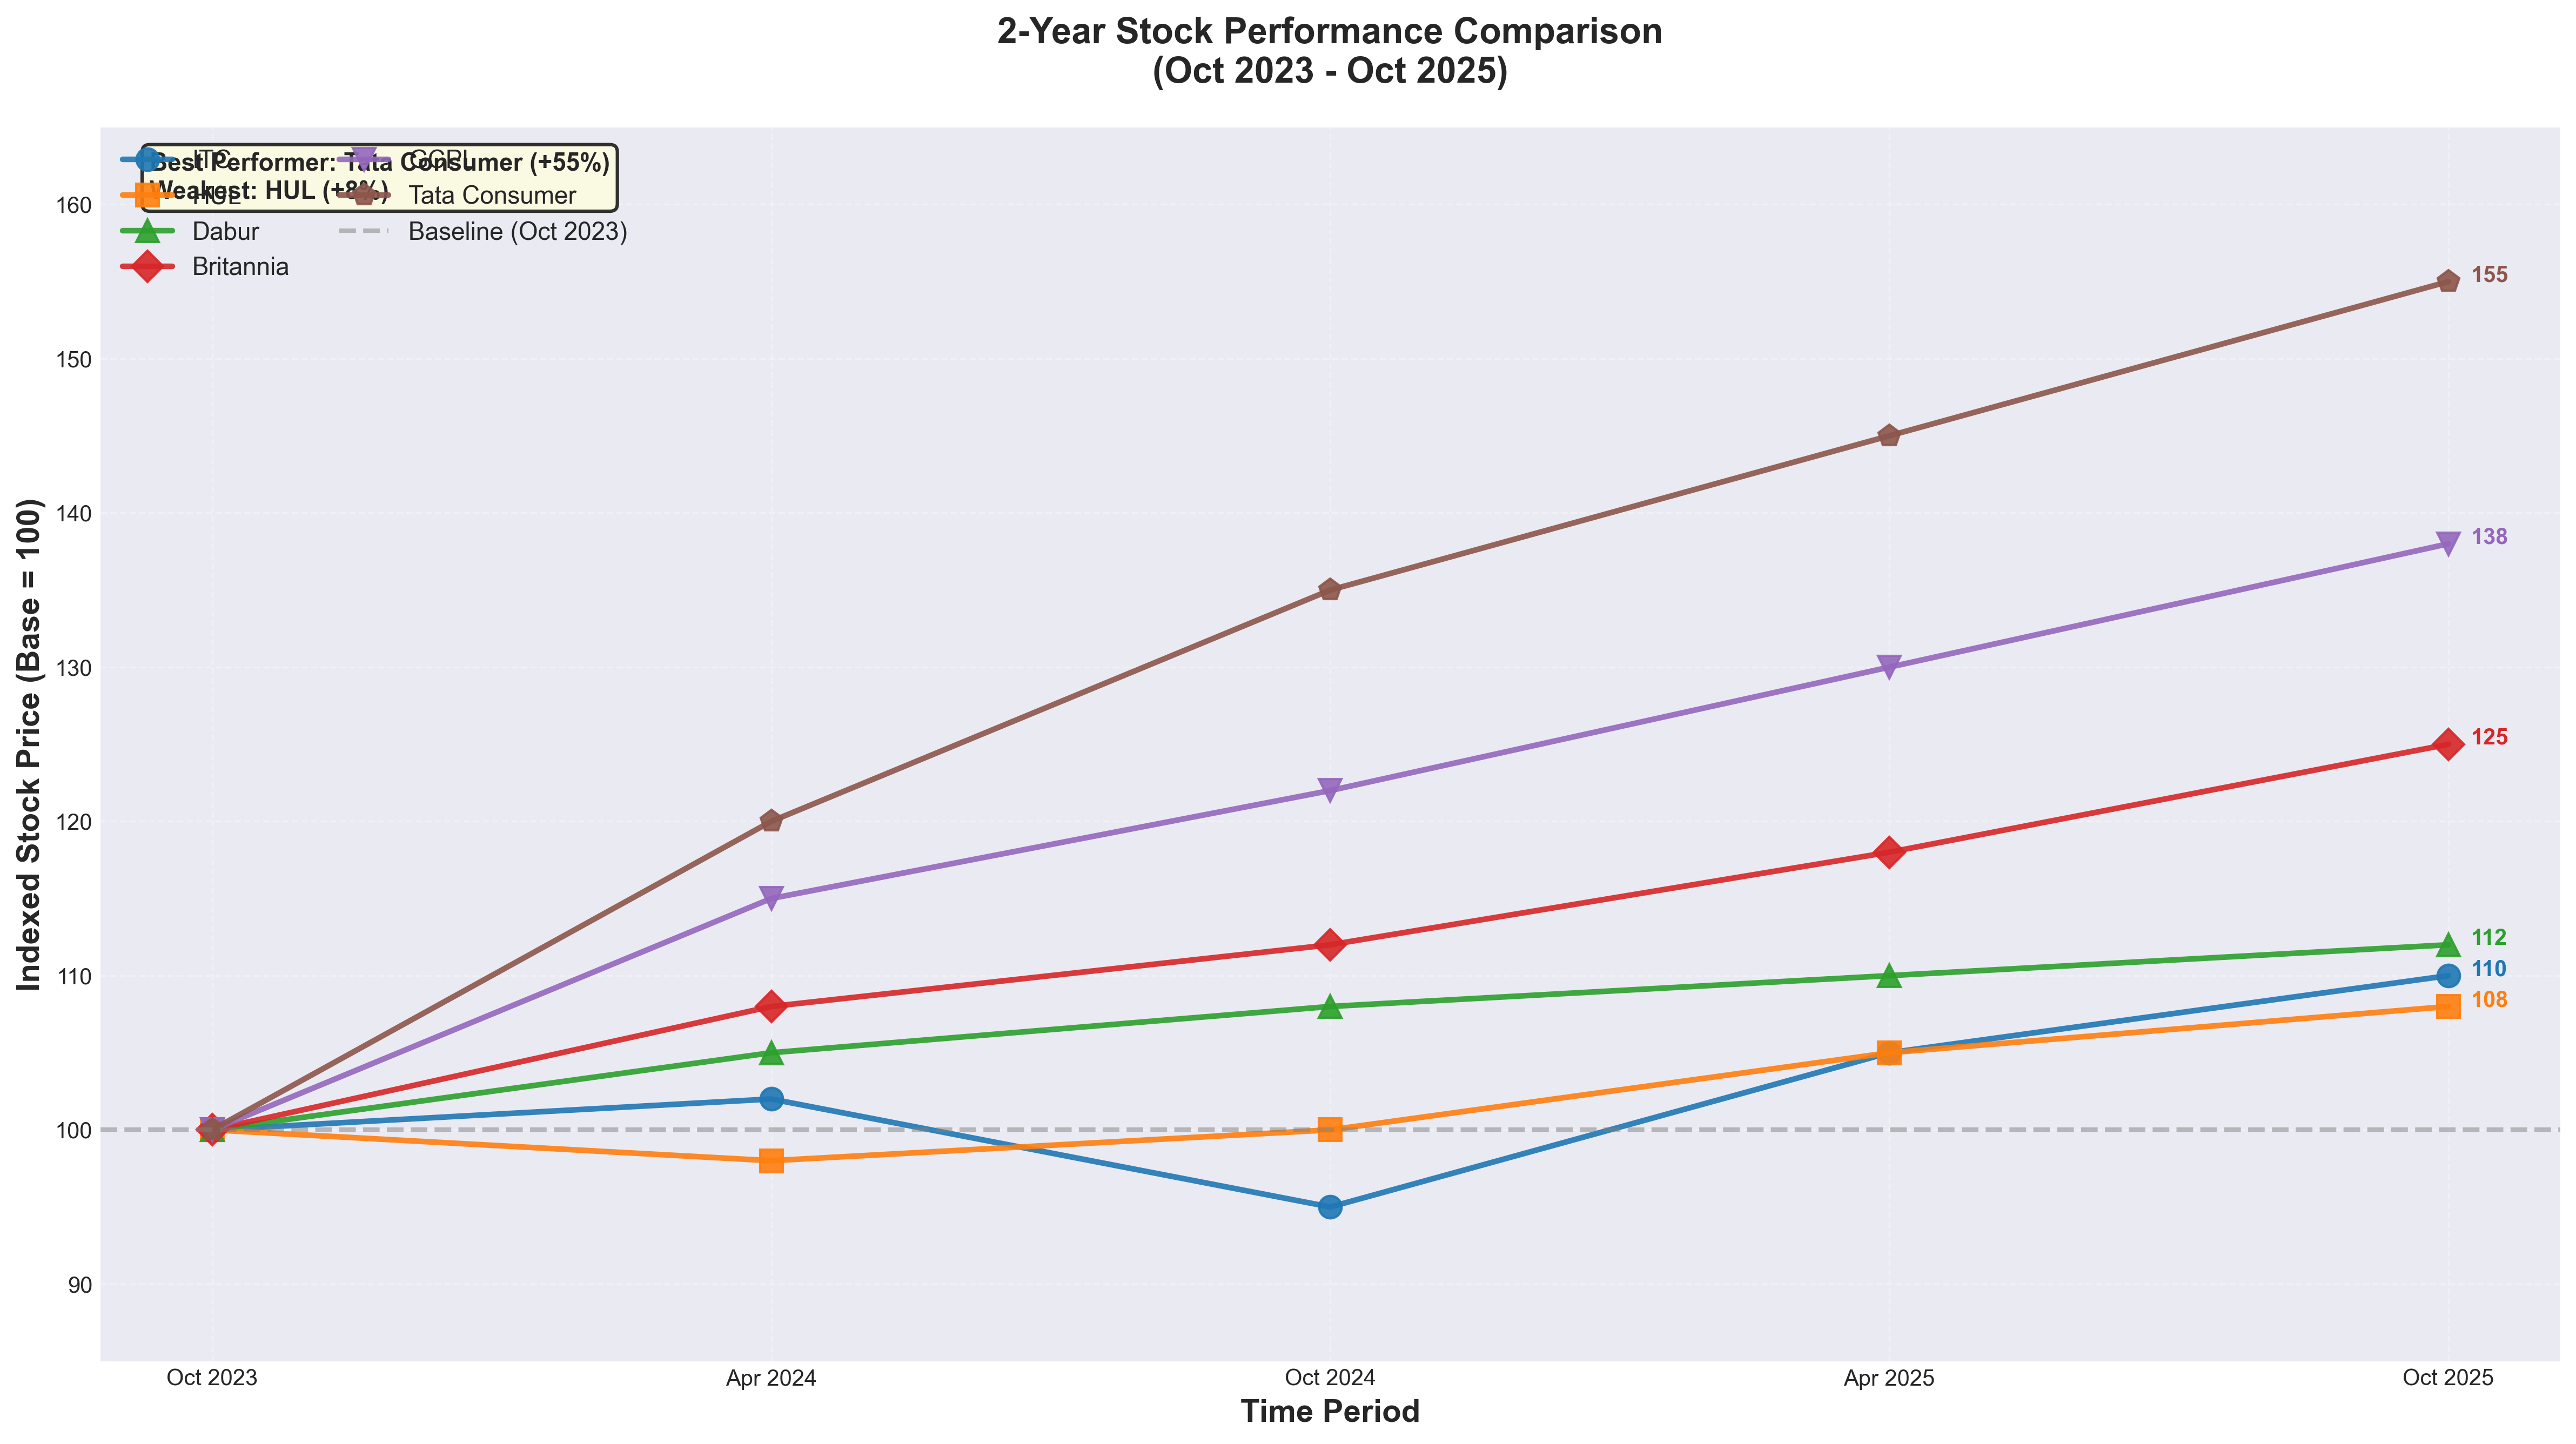
\includegraphics[width=0.85\textwidth]{assets/industry_profile /stock_performance_chart.png}
    \caption{2-Year Stock Performance - Indexed to October 2023 (Base = 100)}
\end{figure}

\subsection{Market Capitalization Distribution}

\begin{figure}[H]
    \centering
    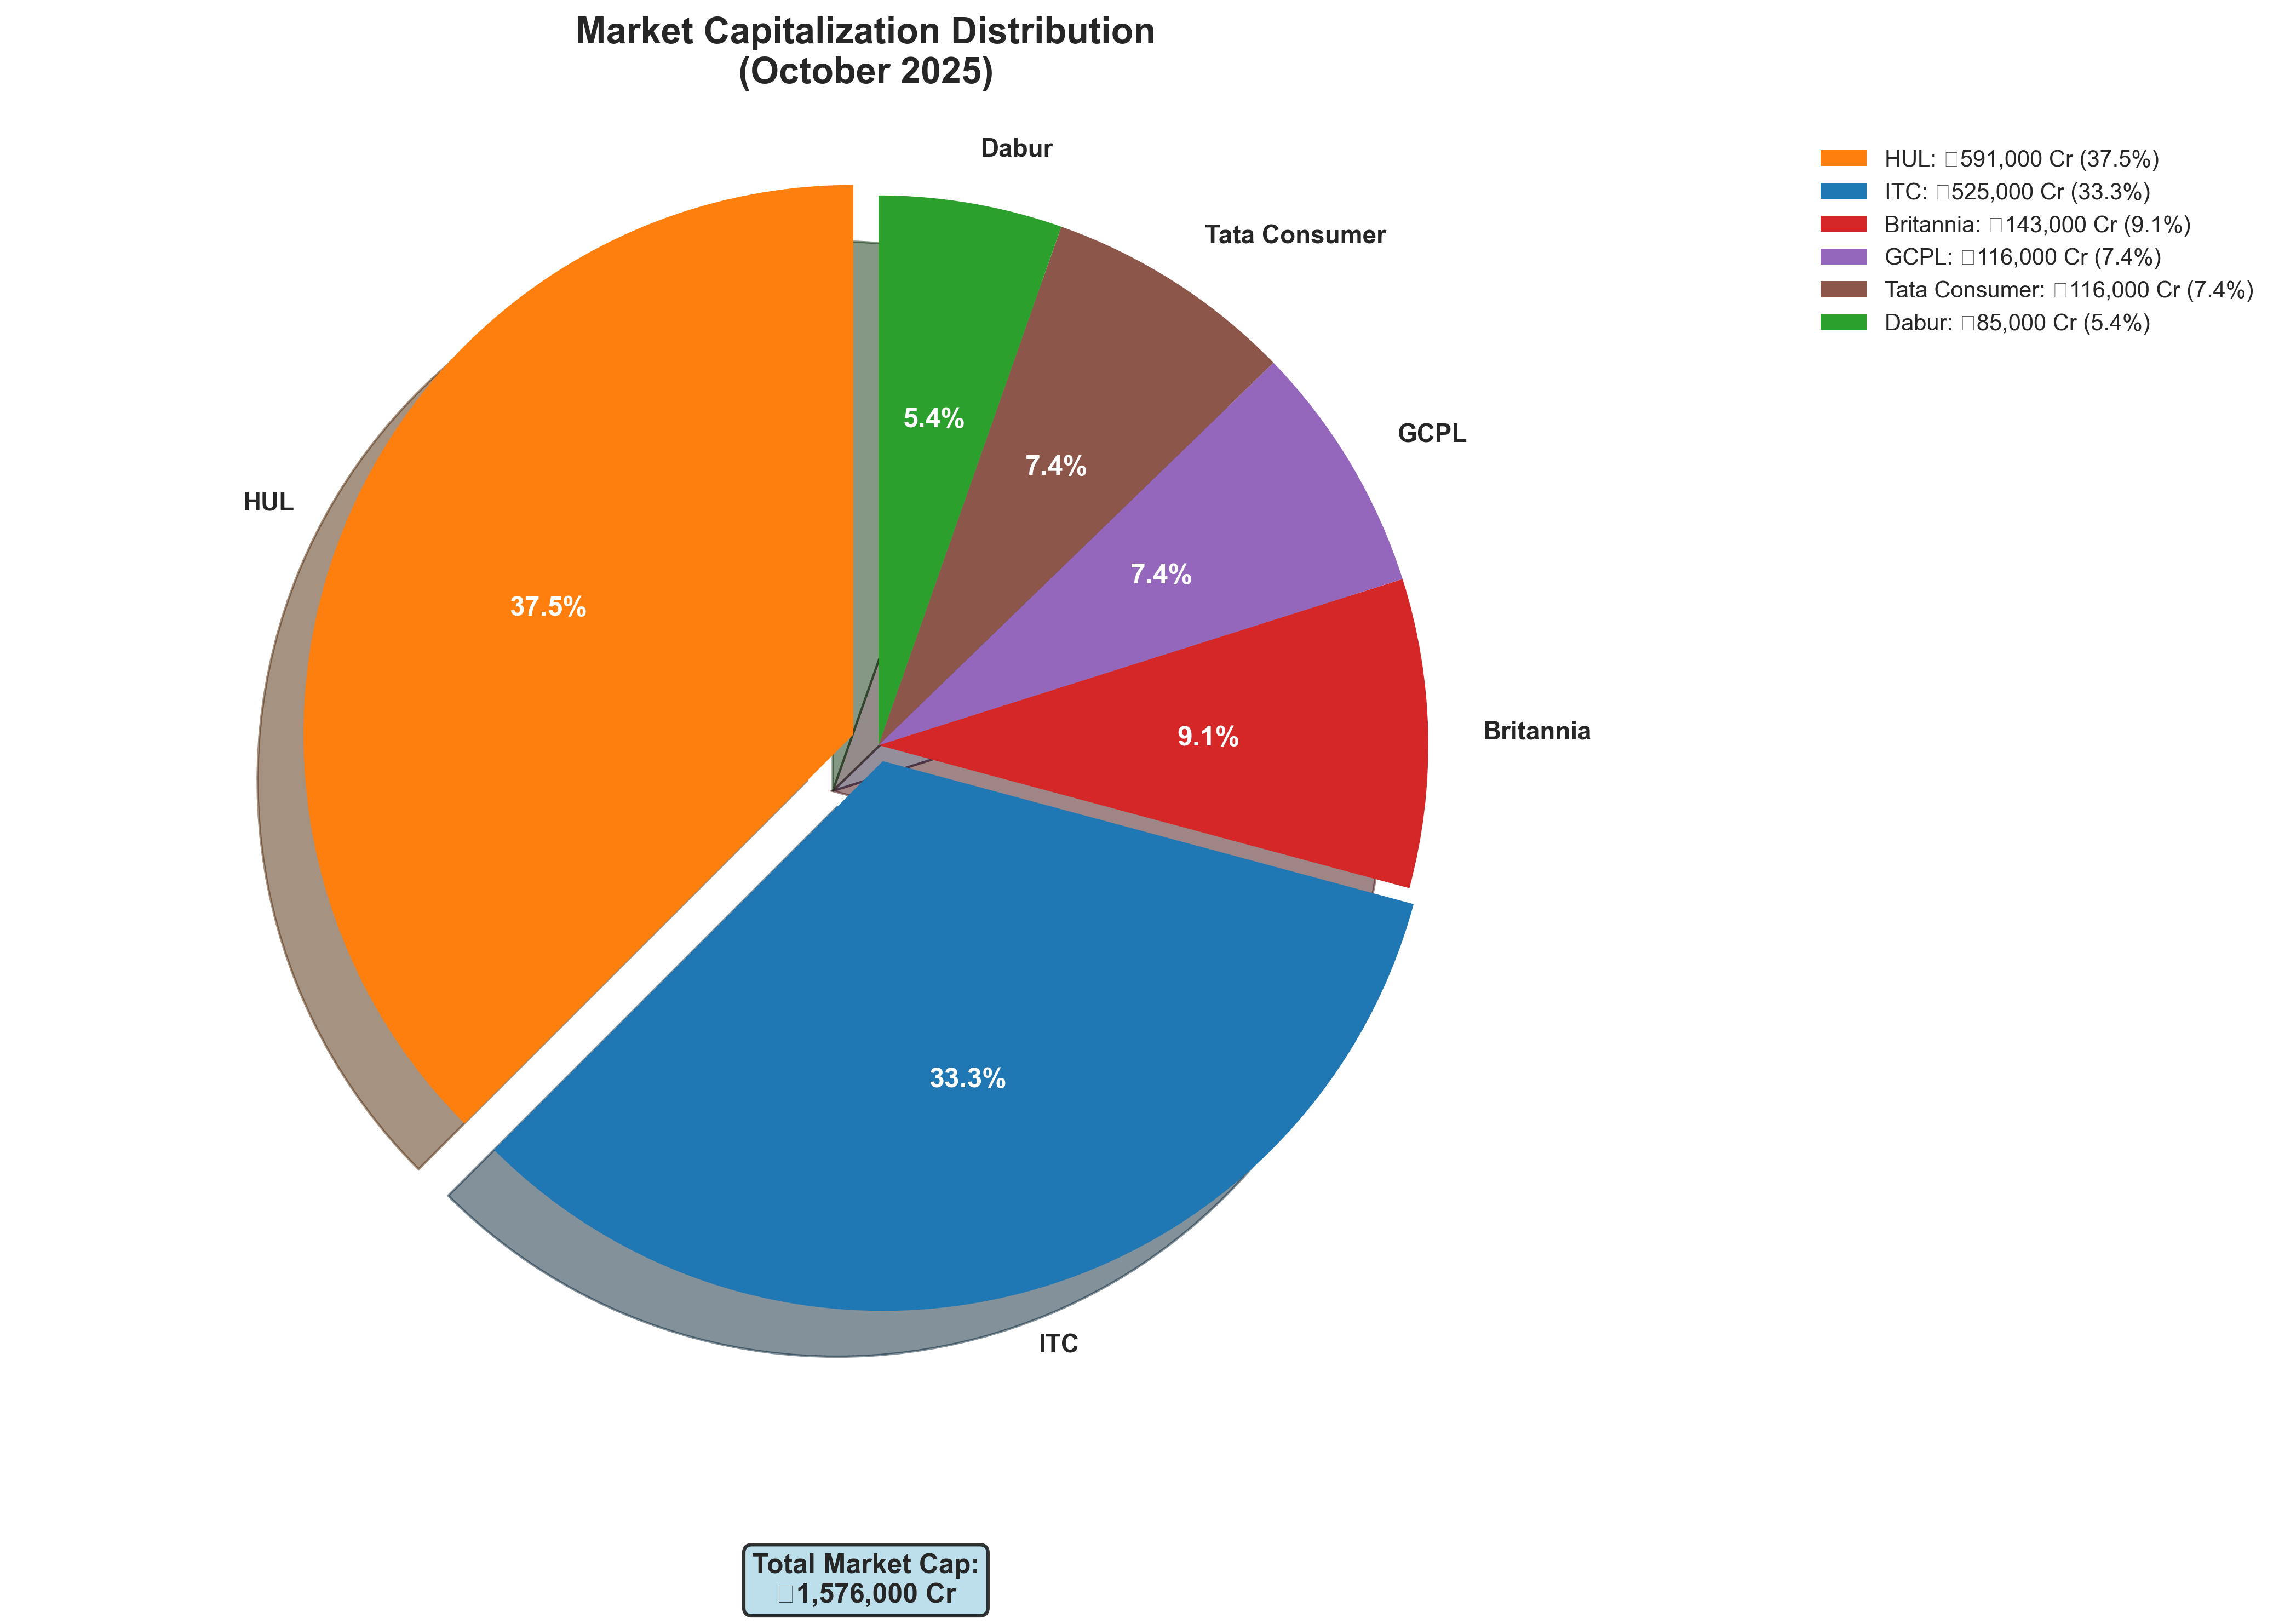
\includegraphics[width=0.85\textwidth]{assets/industry_profile /market_cap_chart.png}
    \caption{Market Capitalization Distribution - October 2025}
\end{figure}

\section{Company Positioning}

\subsection{Tata Consumer Products}

\textbf{Position:} High-growth, high-premium stock. The company's stock surge (+55\%) and extreme P/E ratio (106.53) are completely disconnected from its low 2024 profitability (7.21\% ROE). This is a classic ``growth story'' driven by aggressive acquisition strategy in 2024.

\subsection{ITC}

\textbf{Position:} Mature, high-profit ``value'' stock undergoing transformation. ITC's low P/E (26.13) reflects its legacy as a mature (but highly profitable) tobacco business that pays a high dividend. Stock volatility was event-driven by the demerger of its hotel business.

\subsection{HUL}

\textbf{Position:} The stable, mature market leader. HUL's modest stock growth (+8\%) reflects its maturity, with the company struggling with low volume growth in 2024.

\section{NIFTY FMCG Index}

The NIFTY FMCG index is a sectoral benchmark on the National Stock Exchange of India that tracks the performance of 15 leading companies in the fast-moving consumer goods (FMCG) sector, which includes non-durable and mass-consumption products such as food, beverages, personal care, and household items. 

Calculated using the free float market capitalization method, this index reflects the relative market value of its constituent stocks and serves as a crucial tool for benchmarking, launching ETFs, and structured products. Key constituents include industry giants like Hindustan Unilever, ITC, and Nestlé India, whose steady growth and resilience have ensured the index remains vital for investors and portfolio managers tracking trends in India's rapidly evolving consumer market.

\newpage

% ===============================================
% CHAPTER 4: FINANCIAL STATEMENT ANALYSIS
% ===============================================
\chapter{Financial Statement Analysis}

This report analyzes the financial performance of six major FMCG companies (ITC, HUL, Tata, Dabur, Britannia, and GCPL) across key financial dimensions including liquidity, profitability, leverage, and operational efficiency. The analysis reveals divergent strategic paths: while some companies strengthened their balance sheets through deleveraging, others experienced significant operational challenges requiring deeper investigation.

\section{Liquidity Analysis: Short-Term Financial Health}

\subsection{Strong Performers}

ITC maintains exceptional liquidity with a current ratio of 2.91, improving 2.5\% year-over-year. This positions ITC as the sector leader in short-term solvency, providing substantial cushion to weather market volatility. However, the quick ratio declined 4.8\% to 1.89, suggesting increased inventory levels relative to liquid assets—a concern explored further in operational efficiency metrics.

Dabur demonstrated the most impressive liquidity turnaround, with its current ratio surging 40\% from a concerning 0.85 to 1.19. More remarkably, the quick ratio doubled (106.2\% increase) to 0.79. This transformation suggests aggressive working capital management, potentially through accelerated receivables collection or strategic reduction in short-term liabilities. While still below the 1.5 benchmark, the trajectory indicates improving financial flexibility.

\begin{figure}[H]
    \centering
    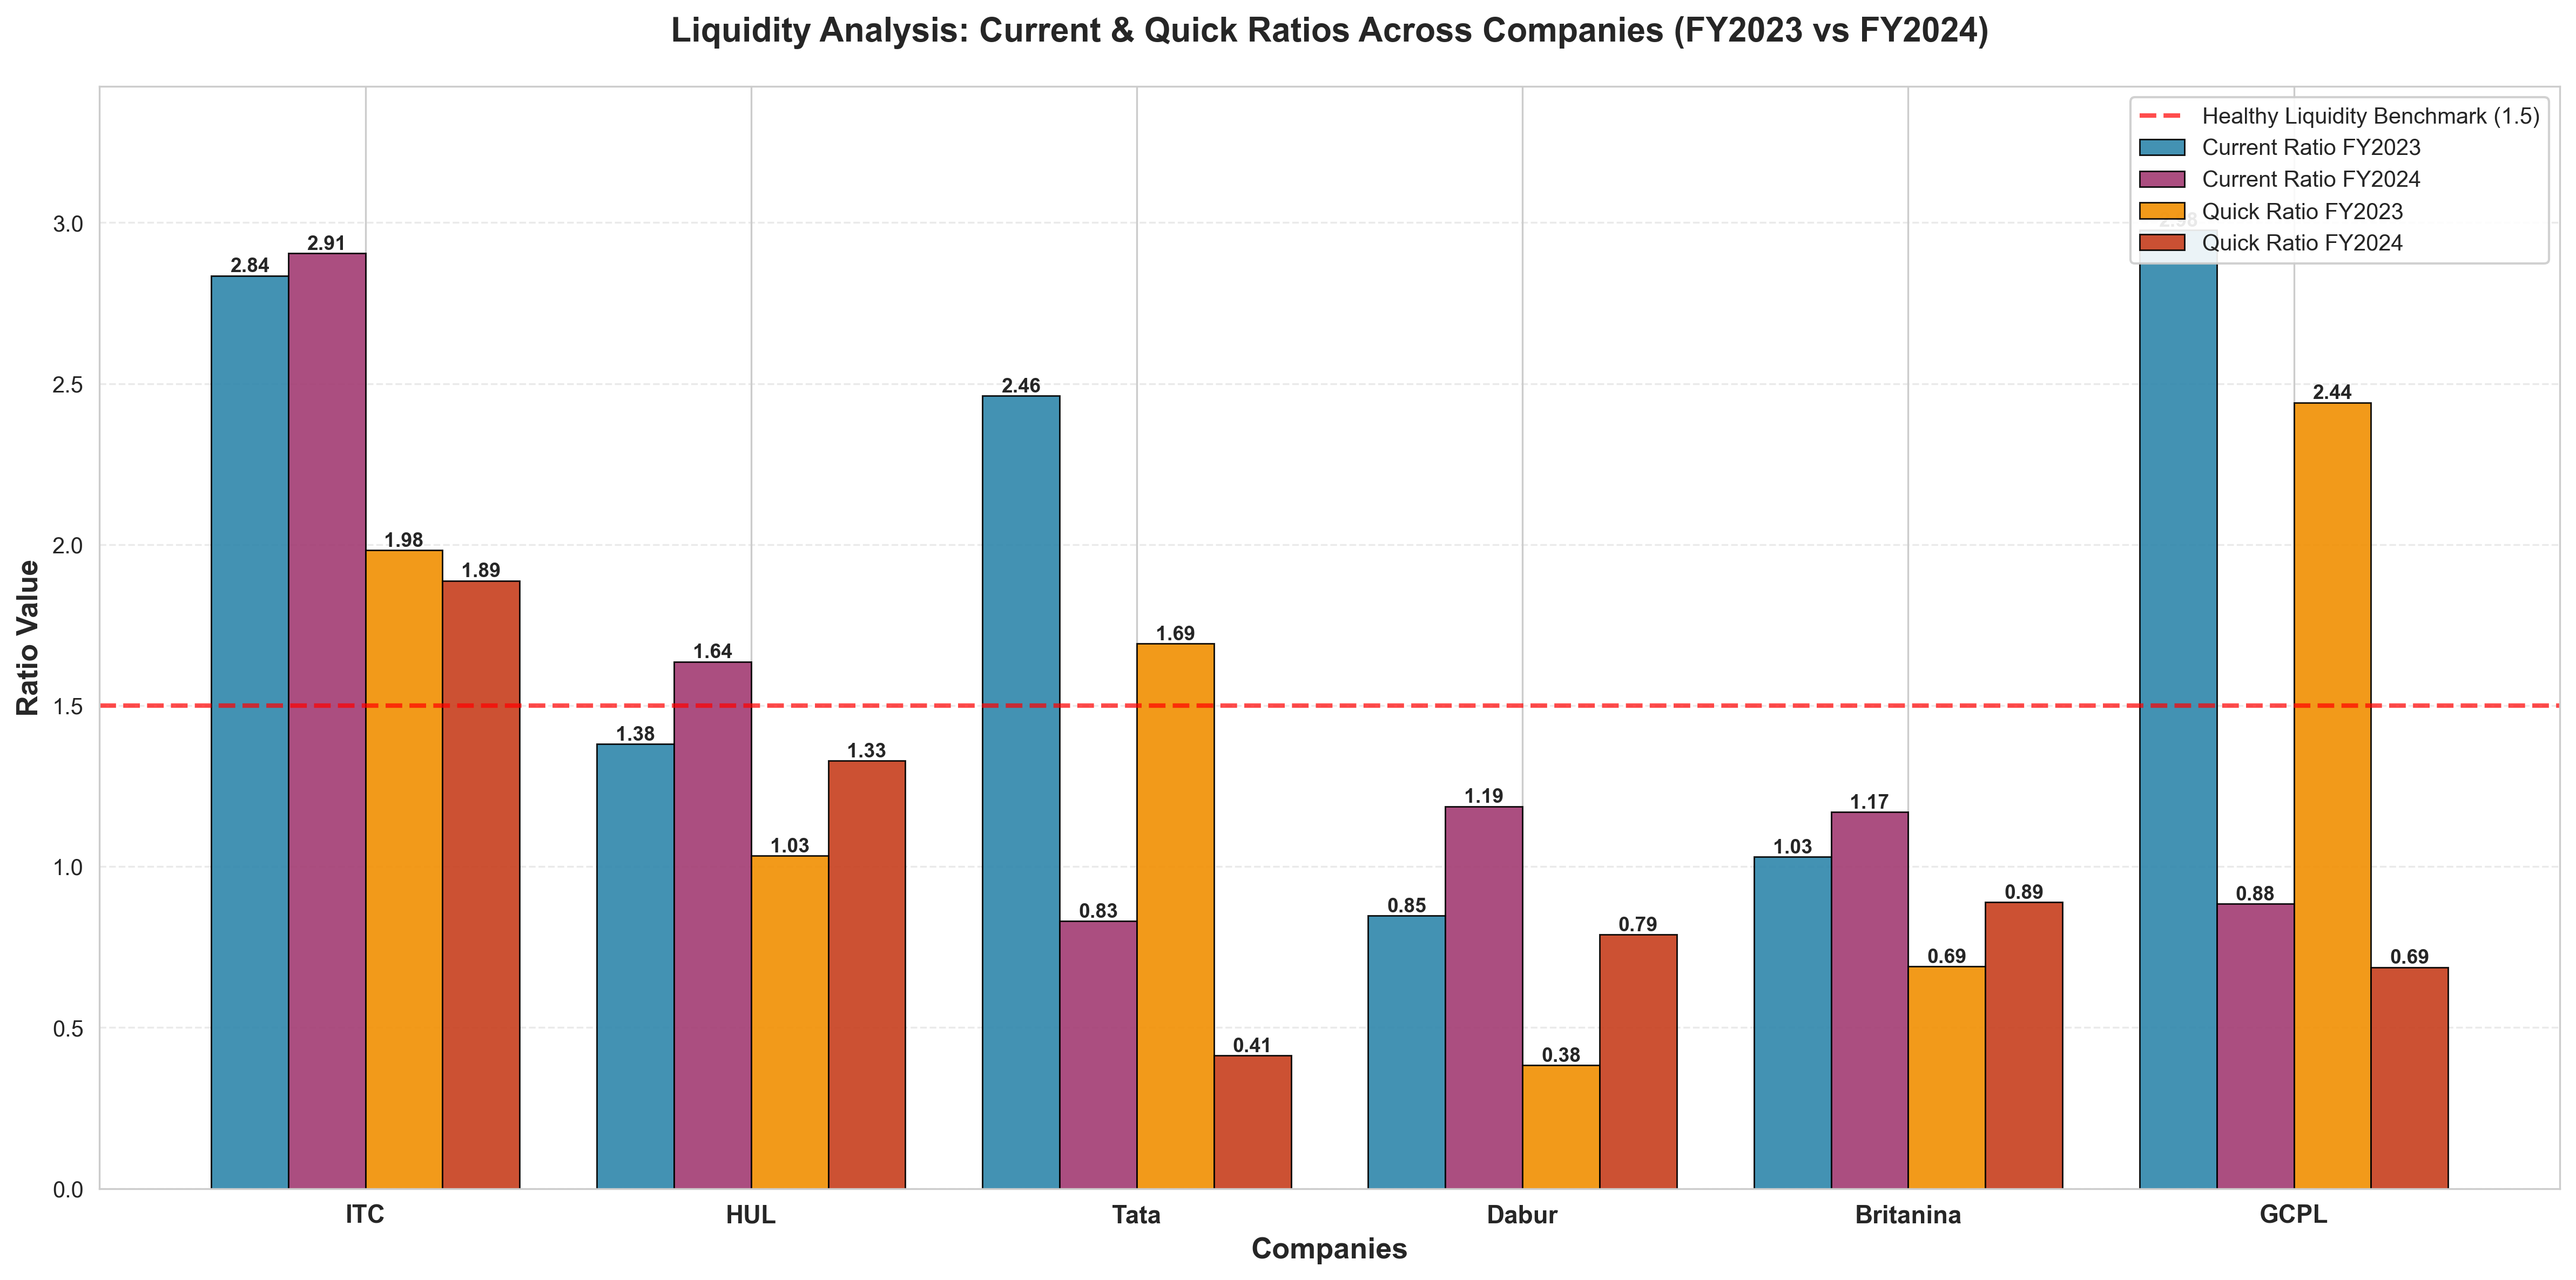
\includegraphics[width=0.8\textwidth]{assets/imperative_analysis/liquidity_analysis.png}
    \caption{Liquidity Analysis - Current and Quick Ratios Comparison}
\end{figure}

\vspace{0.3cm}

GCPL and Tata experienced severe liquidity deterioration that demands immediate management attention. GCPL's current ratio collapsed 70.3\% from 2.98 to 0.88, falling below the critical 1.0 threshold. This dramatic shift, coupled with a 71.8\% decline in quick ratio to 0.69, suggests one of three scenarios: aggressive expansion funded through short-term debt, significant working capital mismanagement, or potential reclassification of liabilities from long-term to short-term.

Tata similarly suffered a 66.2\% liquidity decline (current ratio: 2.46 → 0.83), with quick ratio plummeting 75.6\%. This transformation is particularly alarming given Tata's minimal leverage (D/E: 0.017), suggesting the issue stems from operational factors—possibly inventory buildup or delayed receivables—rather than debt restructuring.

HUL and Britannia occupy the middle ground with modest improvements of 18.6\% and 13.6\% respectively, though both remain below the 1.5 comfort zone at 1.64 and 1.17.

\section{Profitability Analysis: Operational Excellence and Margin Management}

\subsection{Exceptional Performance}

GCPL achieved extraordinary profitability expansion with net profit margin skyrocketing 327.4\% from 17.1\% to 73.0\%. This exceptional jump warrants investigation into whether it reflects: (a) one-time gains from asset sales or restructuring, (b) dramatic cost reduction initiatives, or (c) premium product mix shift. The accompanying 23.9\% gross margin improvement (44.4\% → 55.1\%) suggests genuine operational improvements rather than merely financial engineering, though such extreme growth is unsustainable.

\begin{figure}[H]
    \centering
    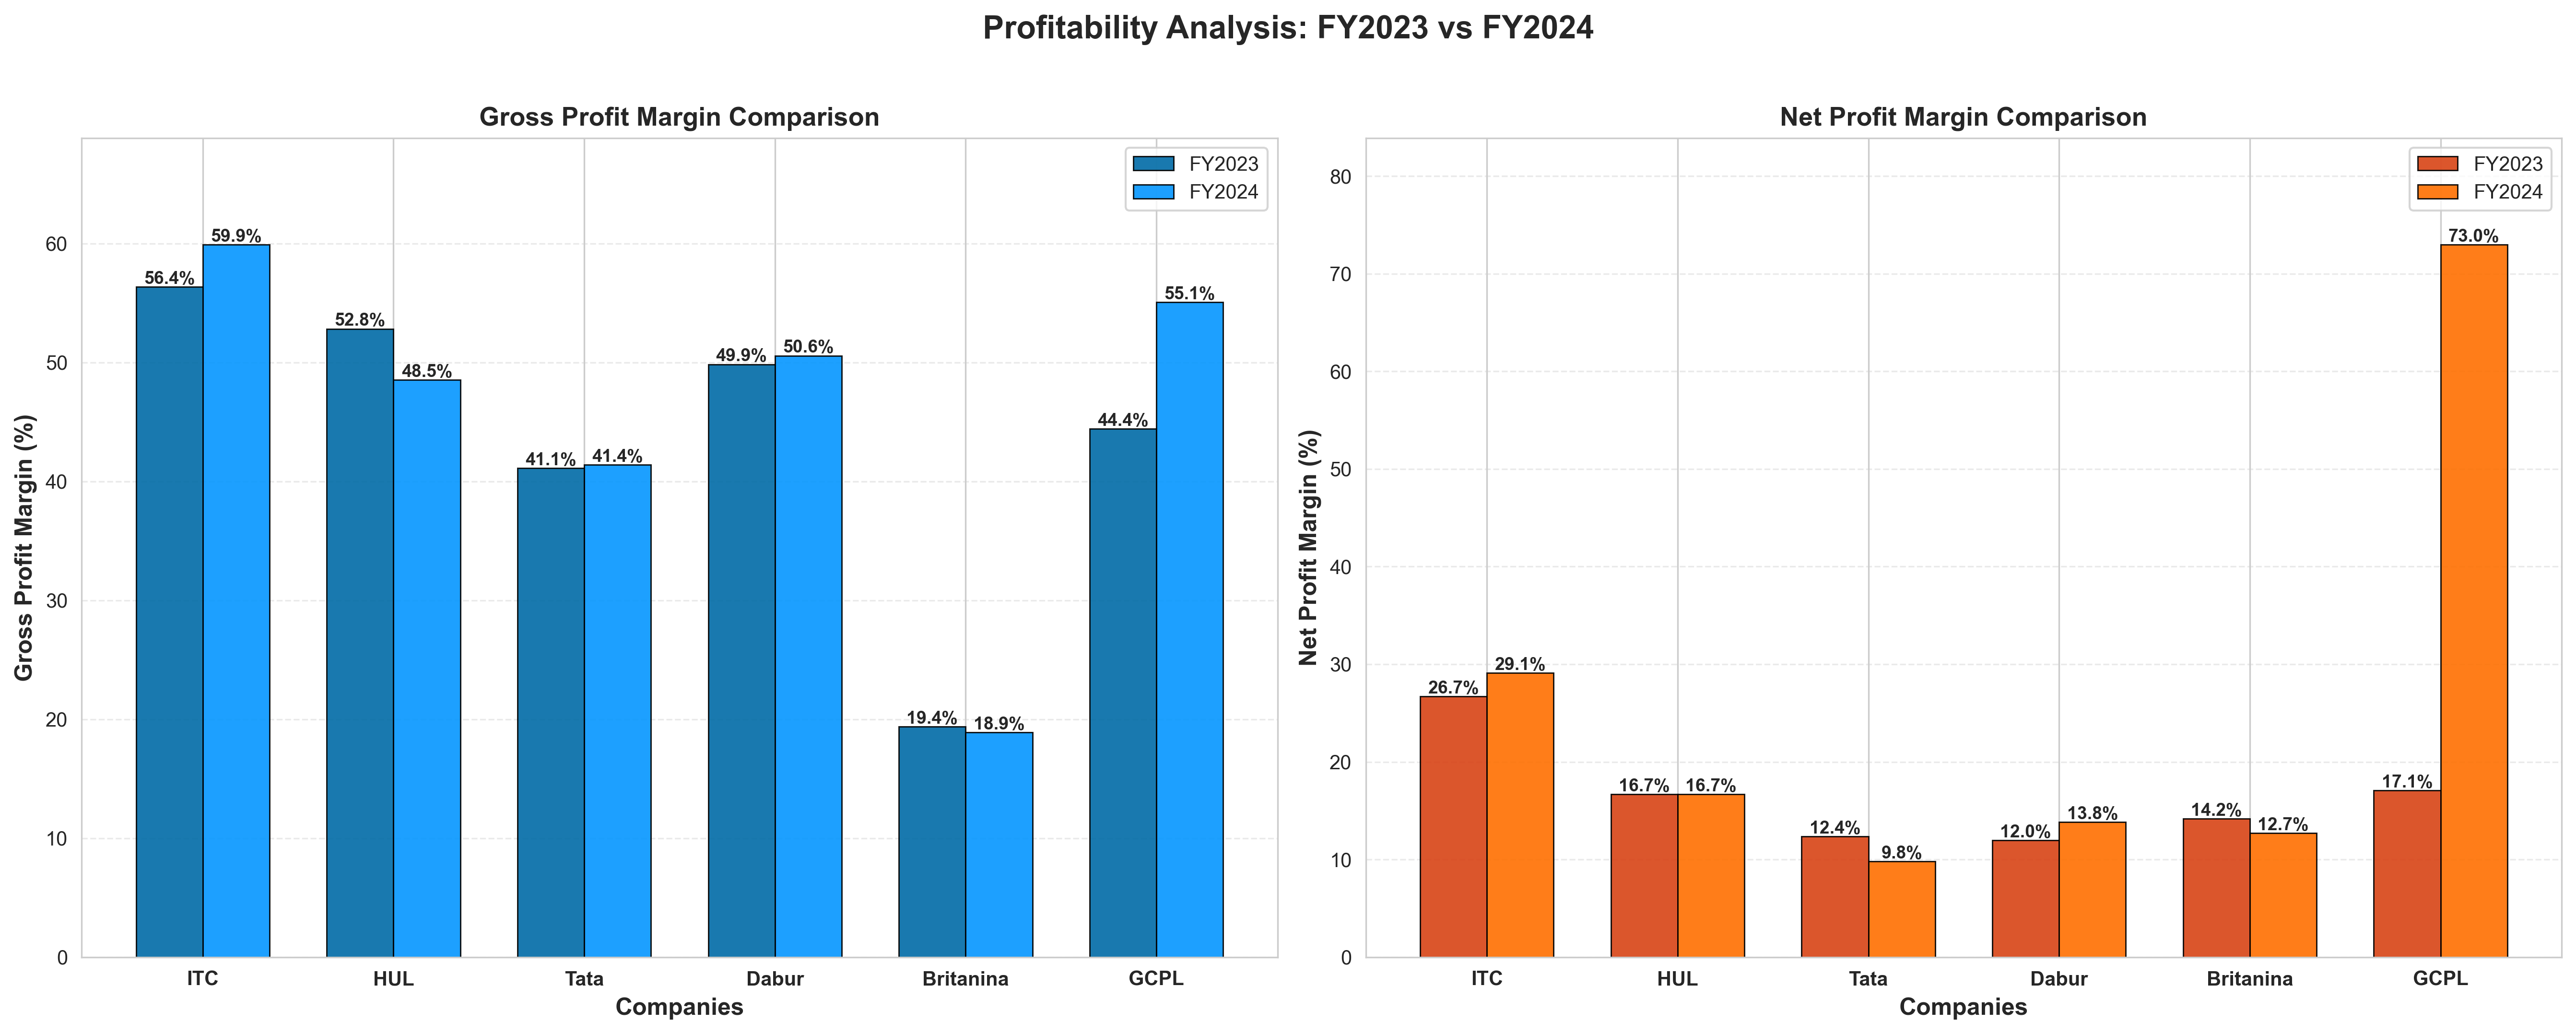
\includegraphics[width=0.8\textwidth]{assets/imperative_analysis/profitability_analysis.png}
    \caption{Profitability Analysis - Net Profit Margins Across Companies}
\end{figure}

\vspace{0.3cm}

Dabur improved net profitability by 15.5\% to 13.8\%, accompanied by modest gross margin expansion of 1.5\%. This balanced improvement suggests effective cost management throughout the value chain rather than dependence on top-line pricing actions alone.

\subsection{Profitability Pressures}

Tata experienced significant msargin compression with net profit declining 20.8\% to 9.8\%, despite maintaining stable gross margins (41.1\% → 41.4\%). This divergence between gross and net margins indicates escalating operating expenses or interest costs consuming the gross profit. The stable gross margin rules out raw material inflation or pricing pressure, pointing instead to SG\&A bloat, increased depreciation, or expansion-related expenses.

Britannia faced a 10.6\% net margin decline to 12.7\%, coupled with a 2.6\% gross margin contraction. This suggests dual pressures: input cost inflation eroding gross profitability, compounded by additional operating expense burdens. As a biscuit manufacturer, Britannia faces direct exposure to wheat, sugar, and palm oil price volatility.

HUL presents an interesting case with net margins remaining virtually flat at 16.7\% (+0.2\%), despite an 8.2\% gross margin decline (52.8\% → 48.5\%). This stability amid gross margin compression indicates aggressive operating expense management, likely reflecting restructuring initiatives, distribution efficiency gains, or reduced marketing spend—a potentially risky trade-off between short-term profitability and long-term brand equity.

\begin{figure}[H]
    \centering
    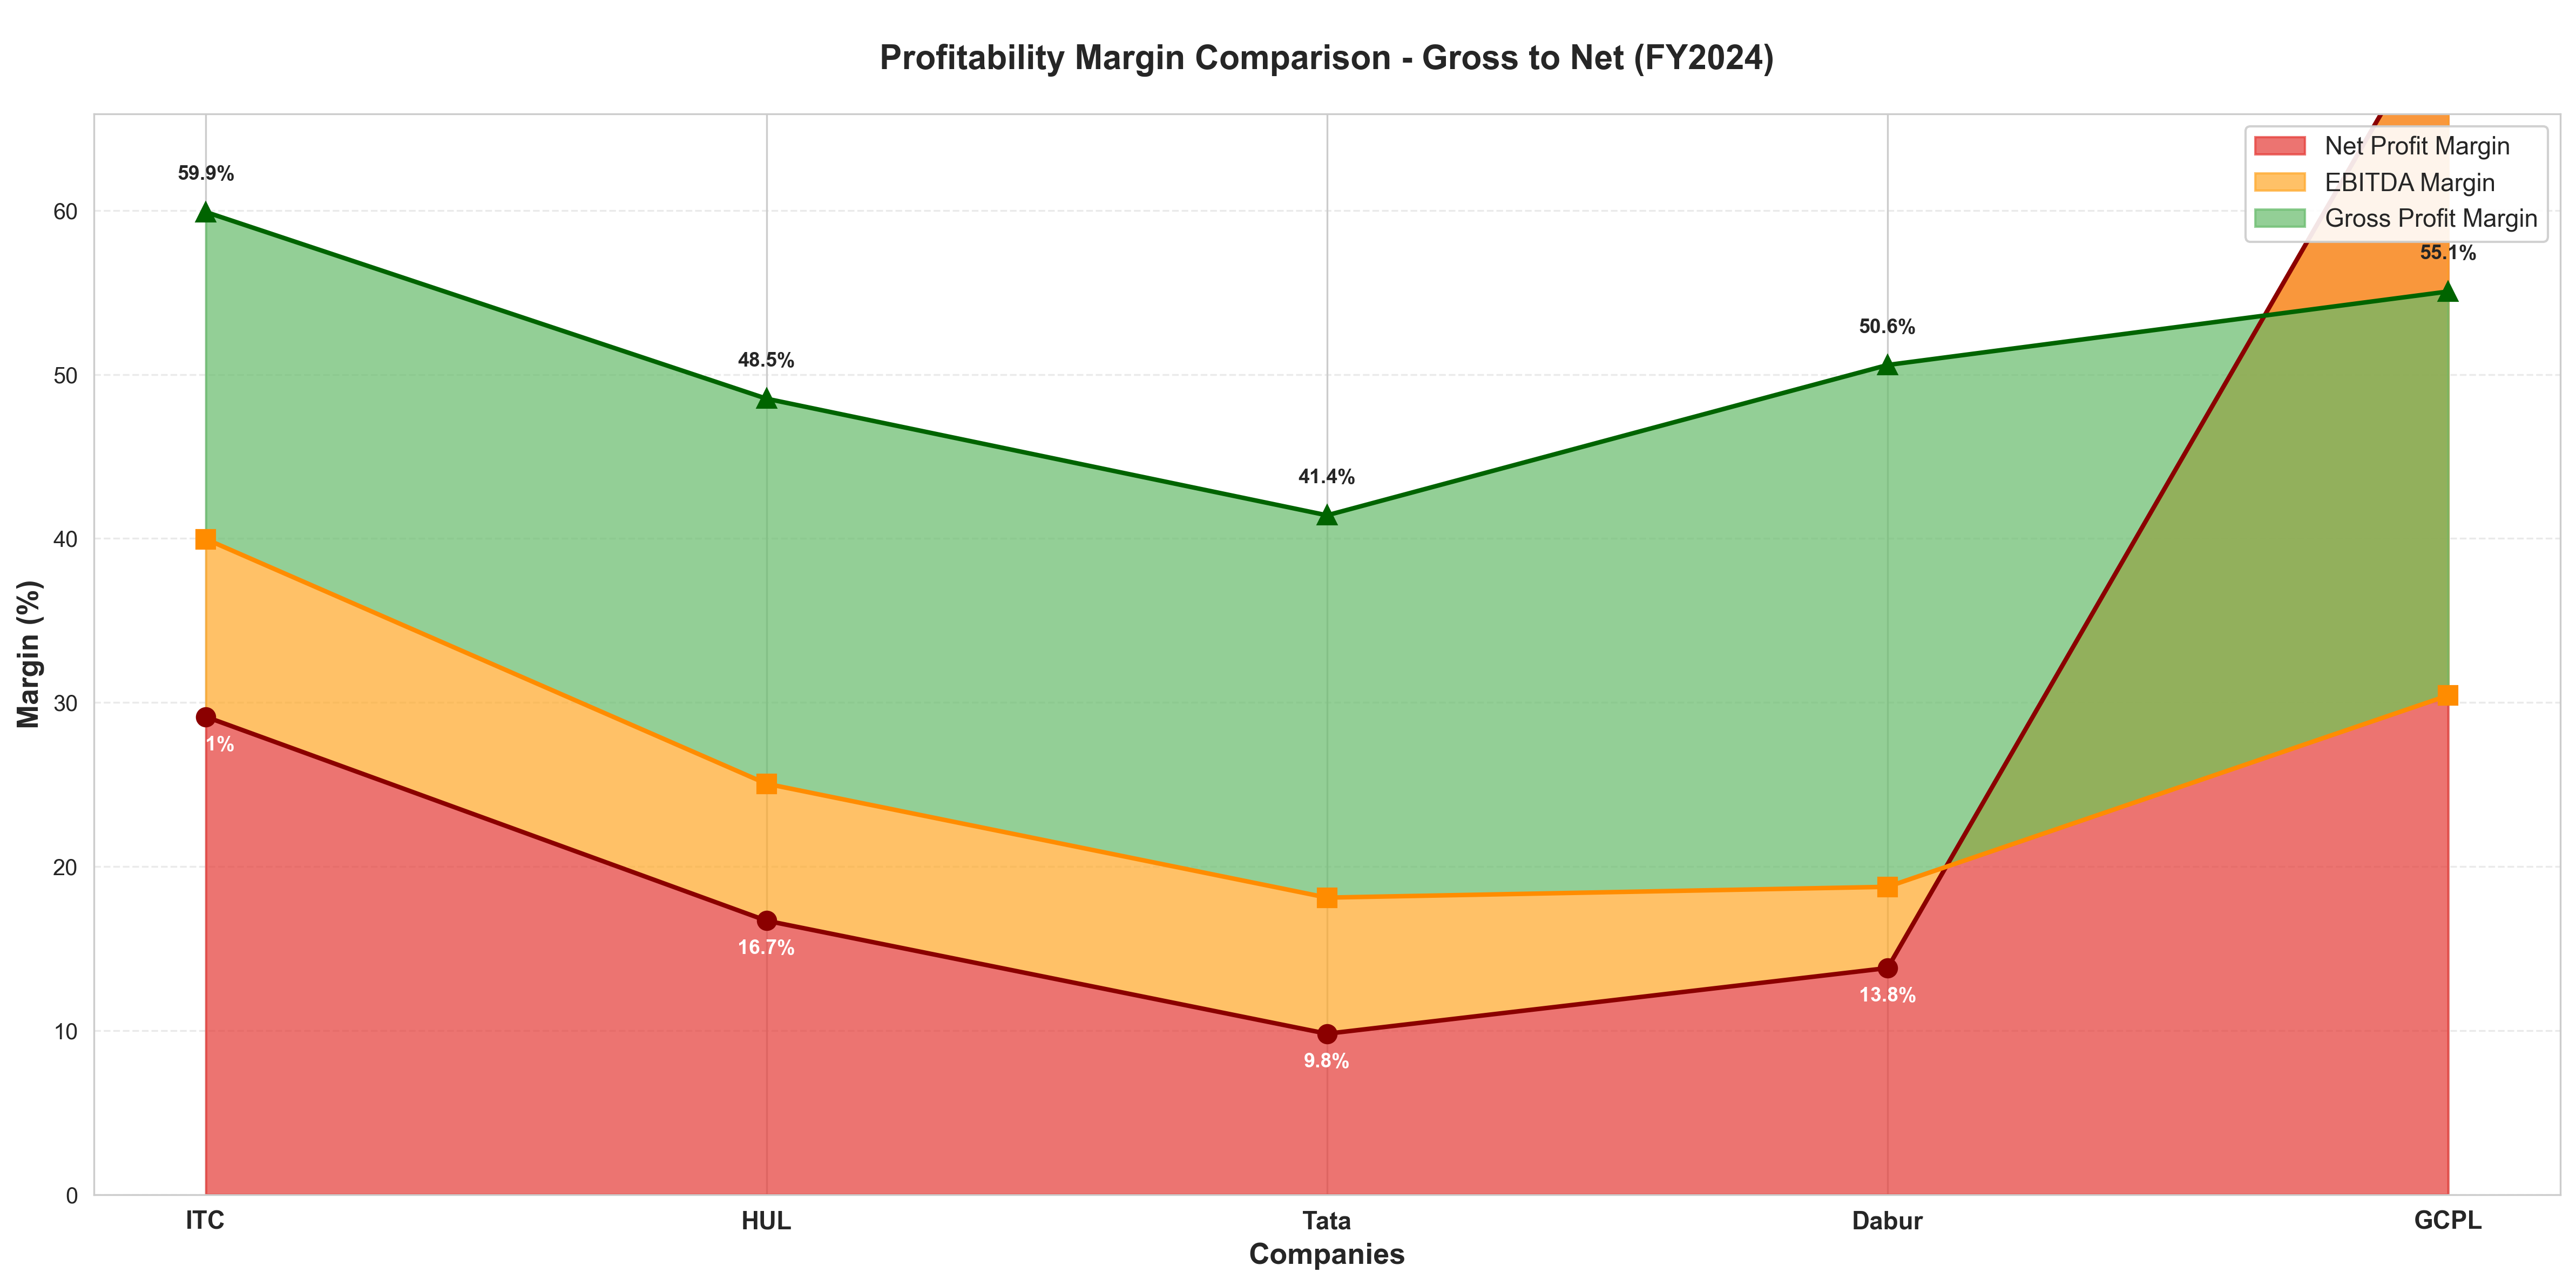
\includegraphics[width=0.8\textwidth]{assets/imperative_analysis/margin_comparison_area.png}
    \caption{Margin Comparison - Gross and Net Margins Across Companies}
\end{figure}

\vspace{0.3cm}

\section{Leverage Analysis: Capital Structure and Financial Risk}

\subsection{Conservative Capital Structures}

ITC maintains a pristine balance sheet with zero debt (D/E: 0.000), reflecting its strong cash generation capacity from tobacco operations. The reported 49.8\% leverage reduction appears to be a data artifact given the zero base.

Britannia executed significant deleveraging, halving its D/E ratio from 0.400 to 0.200 (50\% reduction). This strategic debt reduction, combined with declining profitability, suggests management prioritized financial stability over aggressive growth—a prudent choice for a food company facing volatile commodity markets.

Dabur maintained stable, moderate leverage (D/E: 0.328 → 0.343, +4.8\%), demonstrating disciplined capital allocation while funding operational improvements evidenced by its liquidity and profitability gains.

\subsection{Leverage Build-Up}

GCPL exhibited an astronomical 8,349\% increase in leverage, though the absolute D/E ratio remains conservative at 0.210 (starting from near-zero 0.002). This dramatic relative change likely reflects either debt-funded acquisitions, working capital financing, or capital structure optimization. When considered alongside the 70\% liquidity decline and 327\% profitability surge, this suggests a major corporate event—possibly an acquisition, restructuring, or strategic pivot.

HUL increased leverage 25.3\% (D/E: 0.424 → 0.531), likely reflecting working capital financing or dividend payments exceeding free cash flow. While the absolute ratio remains manageable, the upward trajectory warrants monitoring, especially given gross margin pressures.

Tata showed a modest 12.5\% leverage increase (D/E: 0.015 → 0.017), remaining negligible in absolute terms, suggesting its liquidity challenges stem from operational rather than financial leverage issues.

\begin{figure}[H]
    \centering
    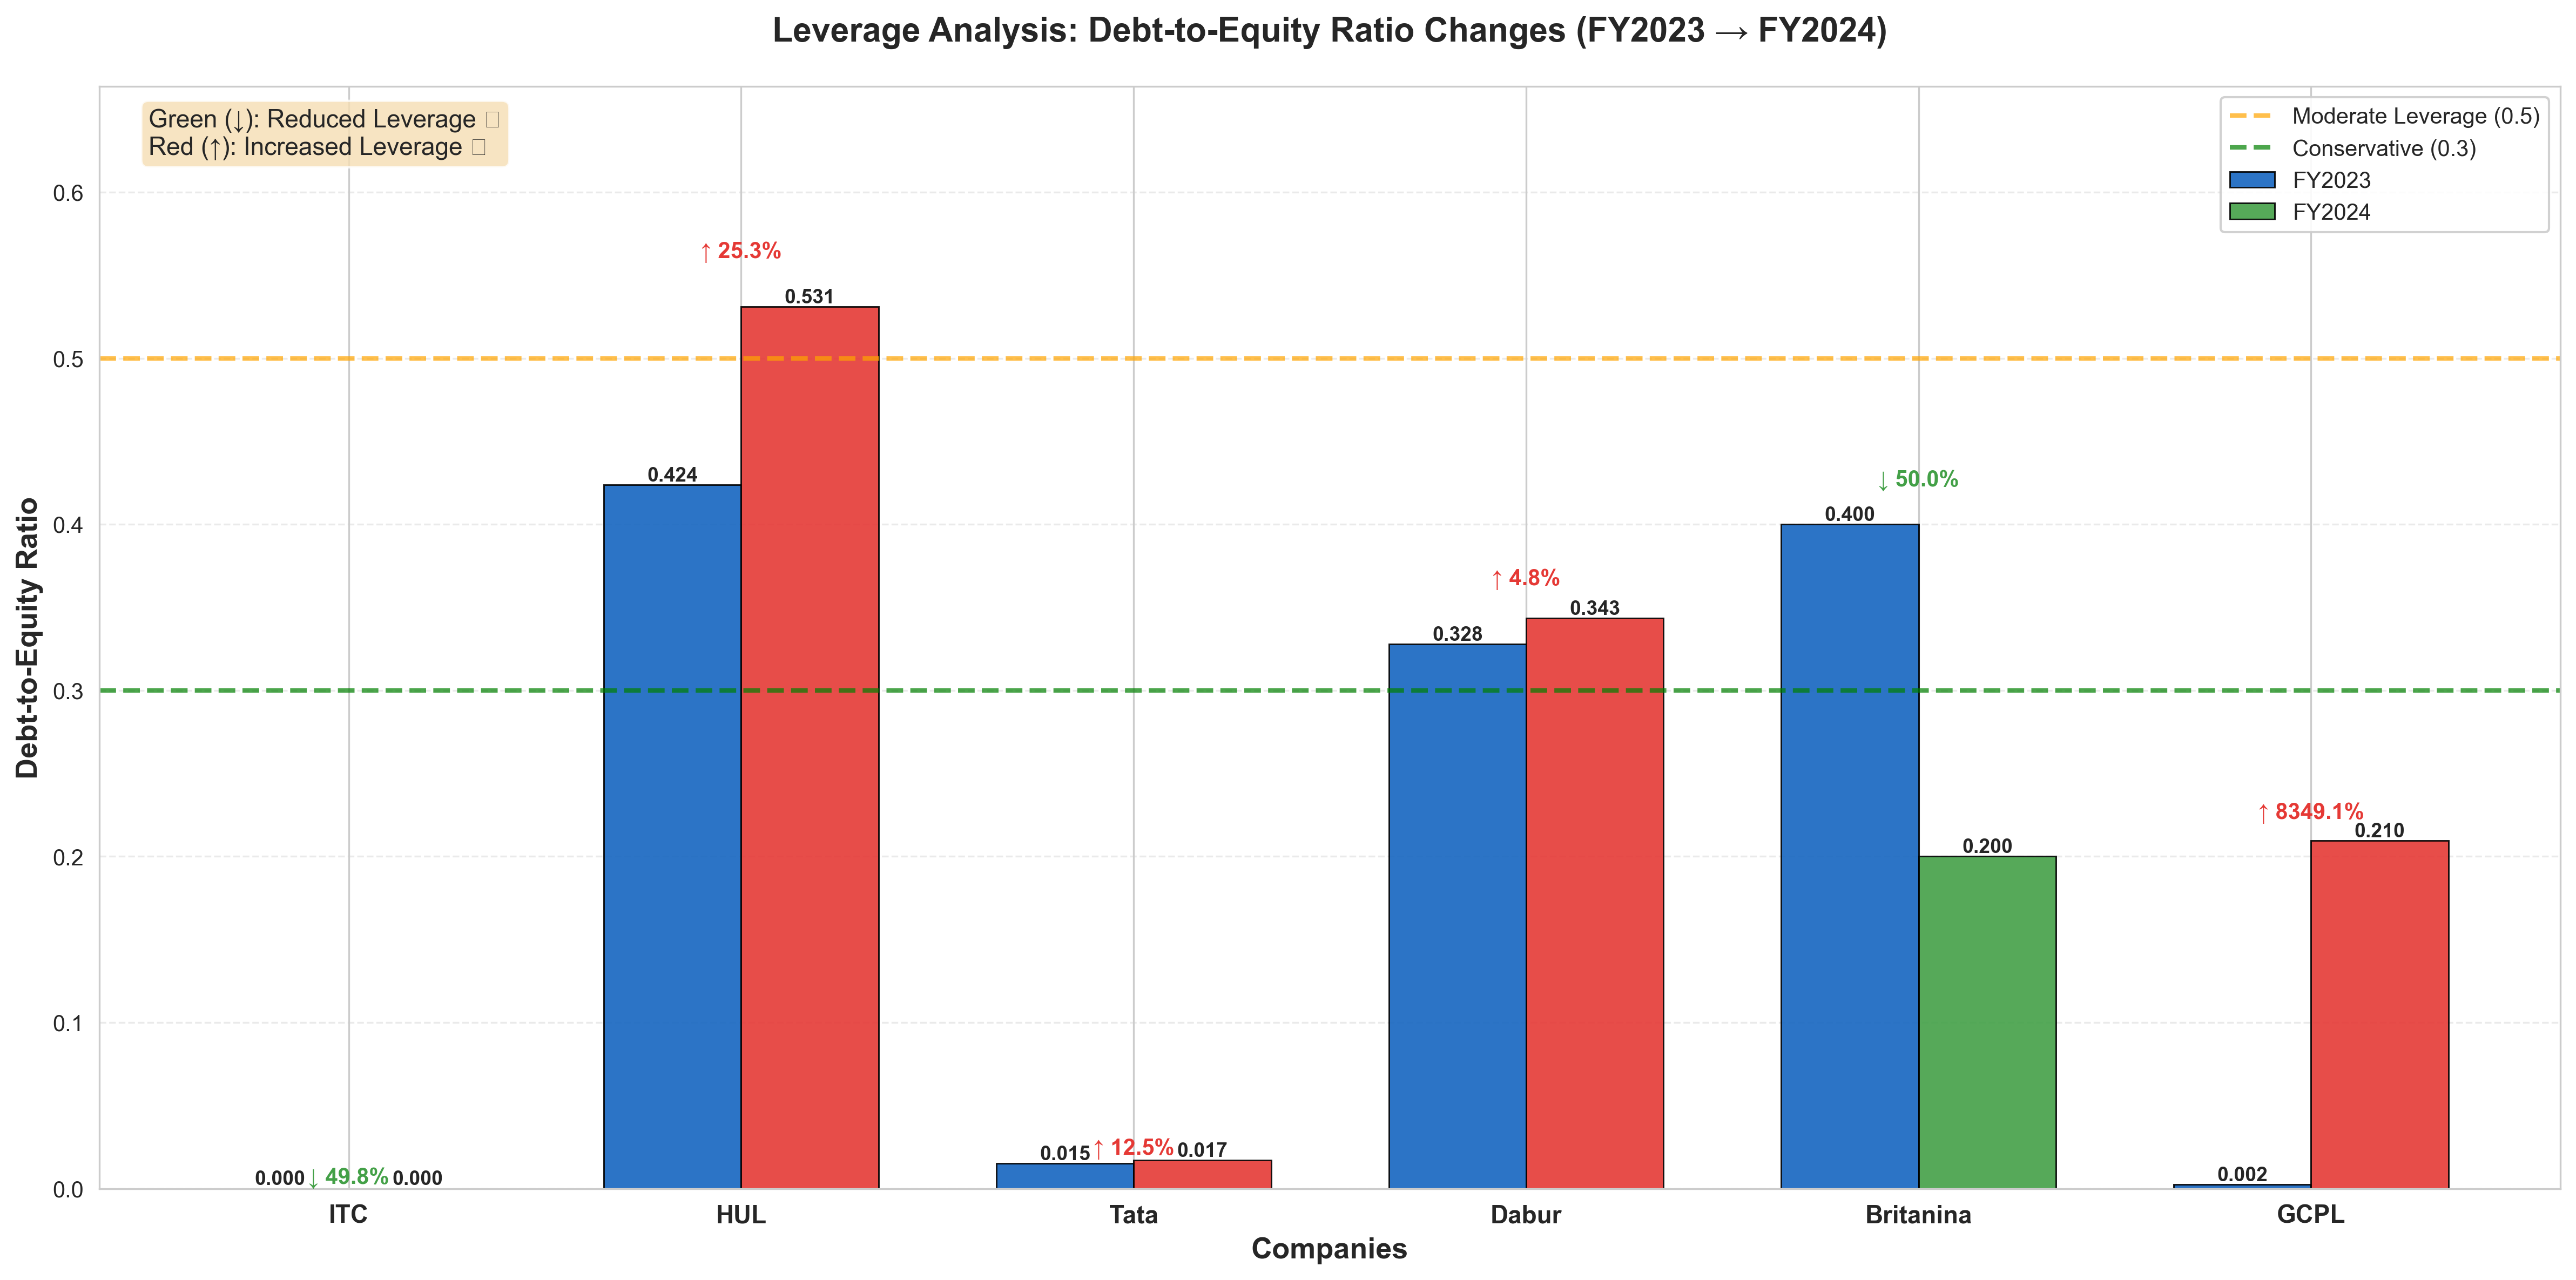
\includegraphics[width=0.8\textwidth]{assets/imperative_analysis/leverage_analysis.png}
    \caption{Leverage Analysis - Debt-to-Equity Ratios}
\end{figure}

\vspace{0.3cm}

\section{Operational Efficiency: Inventory Turnover Analysis}

\subsection{Efficiency Leaders}

Dabur improved inventory turnover 10\% to 5.17x, demonstrating the strongest operational efficiency gains. Combined with improved liquidity and profitability, this suggests comprehensive working capital optimization—faster production cycles, better demand forecasting, or strategic SKU rationalization.

Tata maintained stable, healthy inventory turnover at 3.88x (+0.6\%), indicating consistent operational performance despite profitability pressures and liquidity challenges. This stability suggests Tata's issues lie elsewhere in the working capital cycle, likely in receivables management or payables timing.

\subsection{Efficiency Concerns}

Britannia suffered a dramatic 56.2\% inventory turnover collapse from 15.69x to 6.88x. This severe deterioration, while still above the 5x efficiency threshold, signals potential issues: demand forecasting failures, production over-scheduling, or raw material stockpiling ahead of anticipated price increases. Combined with declining profitability and improving liquidity, this suggests Britannia converted cash into inventory—potentially tying up working capital inefficiently.

ITC experienced a 15.2\% inventory turnover decline to 2.73x, indicating slower stock conversion. For a diversified conglomerate, this could reflect strategic inventory building in hotels (ahead of seasonal demand) or FMCG (anticipating supply chain disruptions), but nevertheless represents capital tied up earning suboptimal returns.

HUL and GCPL lack reported inventory turnover data, preventing comprehensive operational efficiency assessment.

\begin{figure}[H]
    \centering
    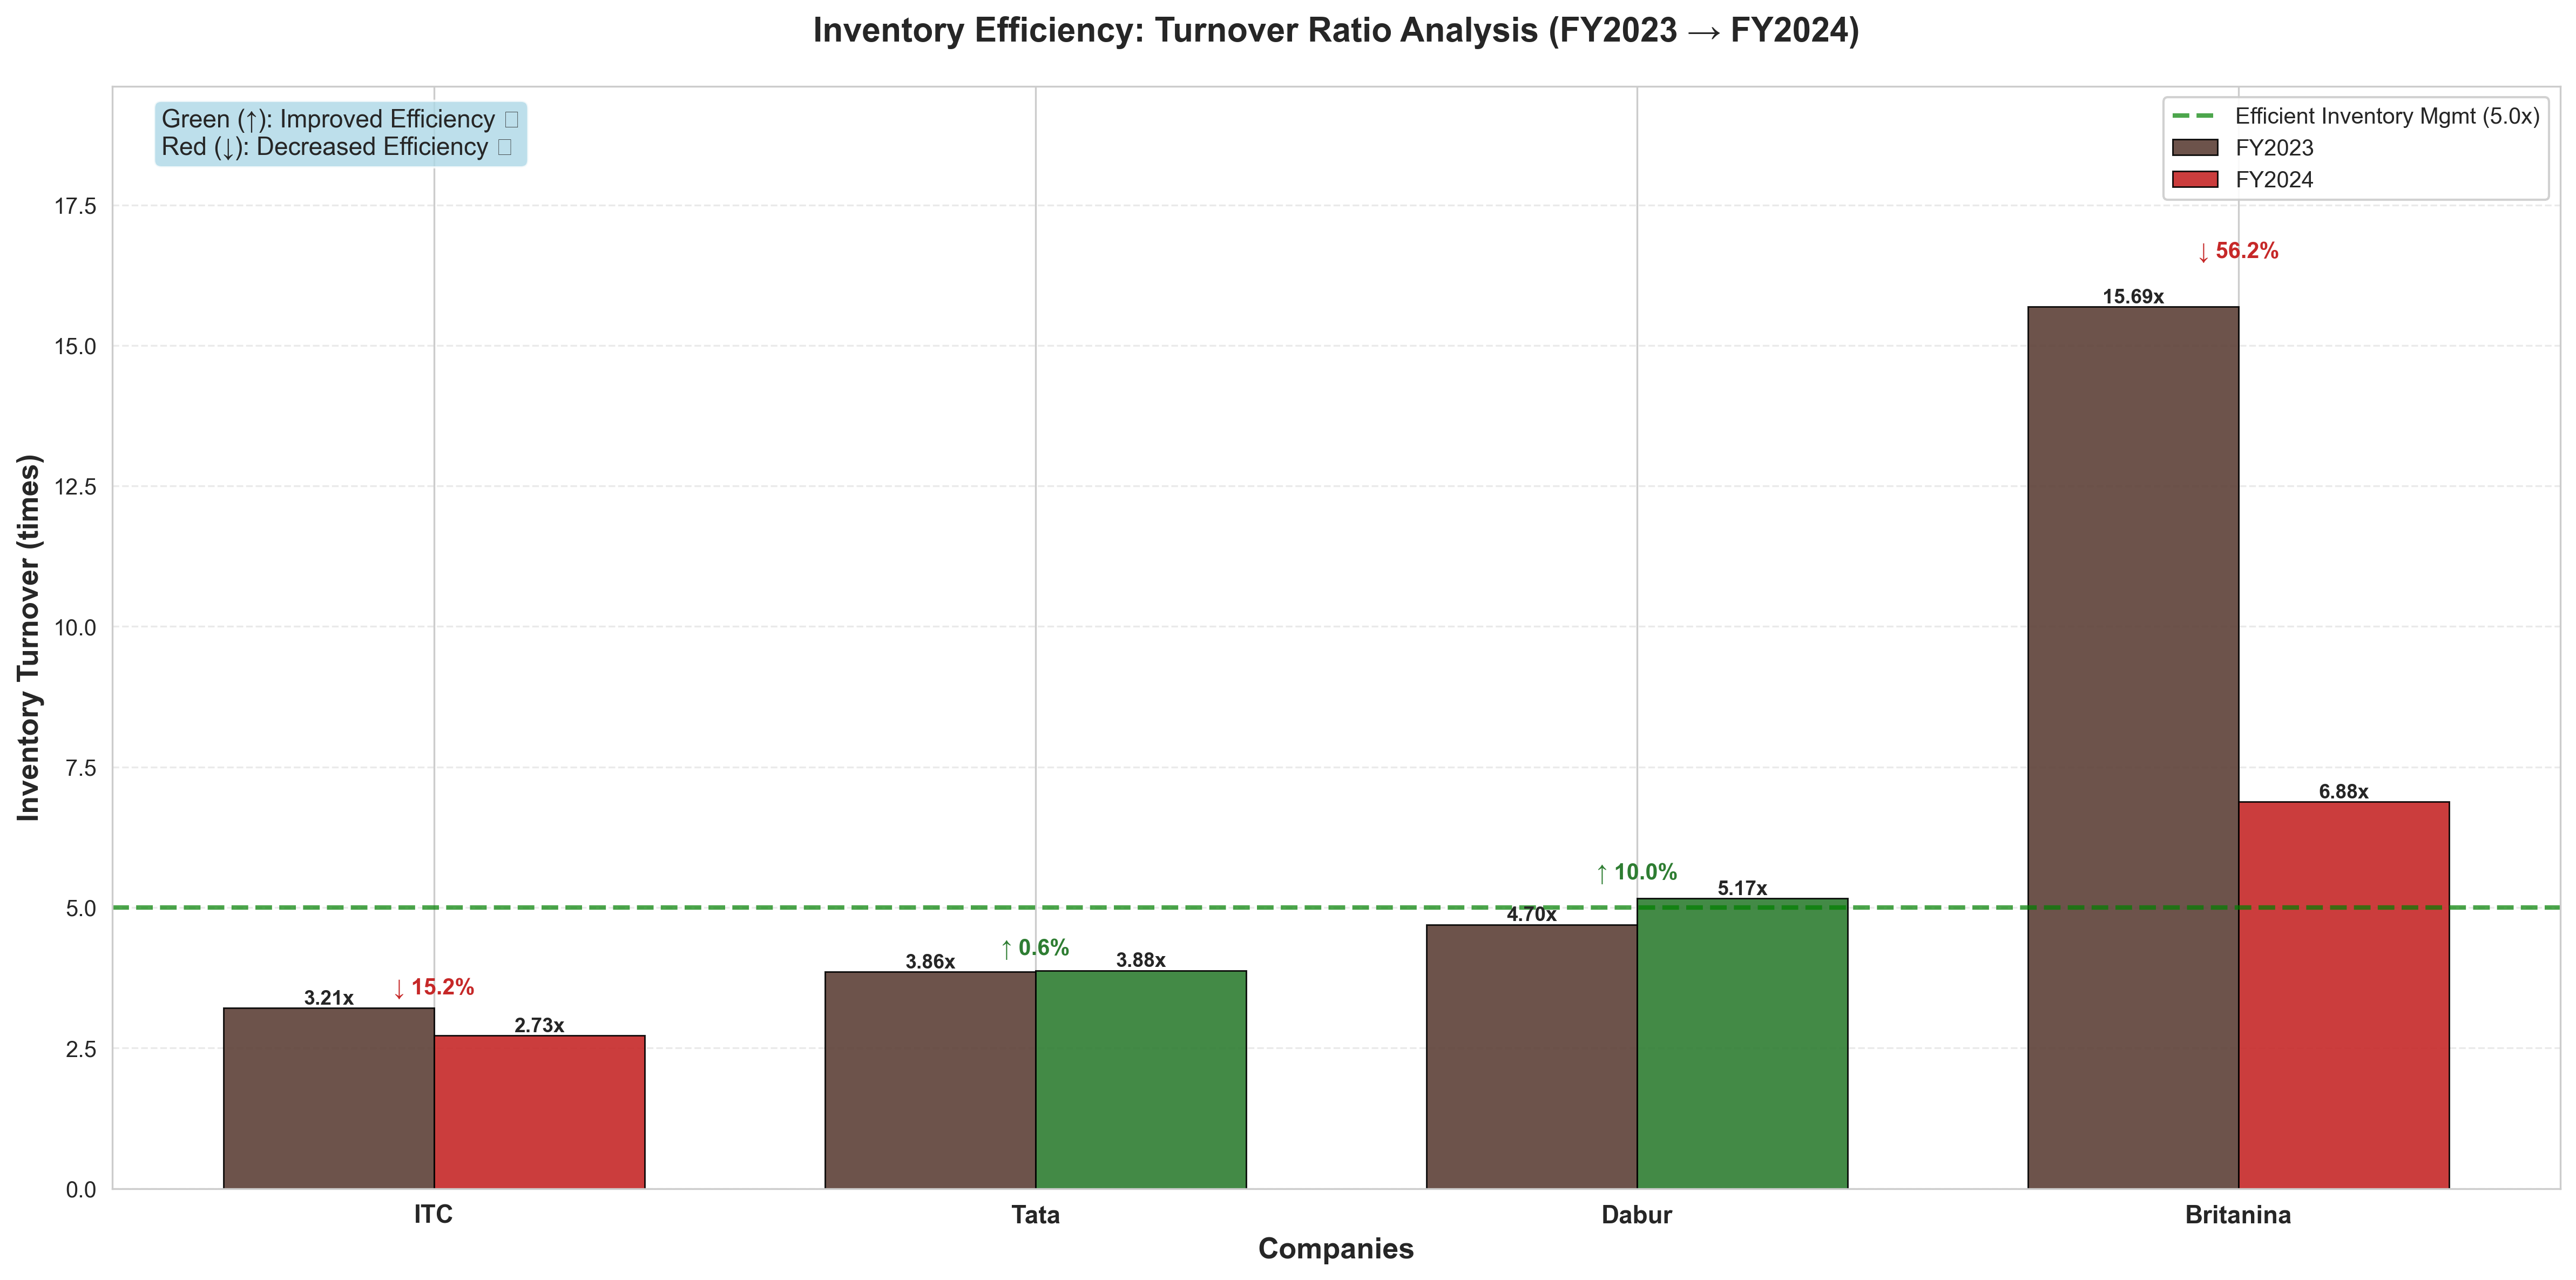
\includegraphics[width=0.8\textwidth]{assets/imperative_analysis/inventory_analysis.png}
    \caption{Inventory Analysis - Turnover Ratios}
\end{figure}

\vspace{0.3cm}

\section{Comparative Rankings and Strategic Positioning}

\subsection{Overall Financial Health Leaders}

\begin{itemize}
    \item \textbf{ITC:} Excellent liquidity (2.91), exceptional profitability (29.1\%), zero debt, though inventory efficiency declined
    \item \textbf{Dabur:} Balanced improvement across all metrics—40\% liquidity gain, 15.5\% profitability increase, 10\% efficiency improvement
    \item \textbf{HUL:} Solid liquidity recovery (18.6\%), stable profitability amid margin pressures, moderate leverage increase
\end{itemize}

\subsection{Companies Requiring Strategic Review}

\begin{itemize}
    \item \textbf{GCPL:} Extreme volatility across all metrics suggests major corporate event requiring investigation
    \item \textbf{Tata:} Severe liquidity crisis (-66\%) despite minimal leverage and stable inventory turnover
    \item \textbf{Britannia:} Profitability and efficiency deterioration despite successful deleveraging
\end{itemize}

\section{Strategic Implications and Recommendations}

\subsection{For Strong Performers (ITC, Dabur)}

These companies should leverage their financial strength for strategic initiatives: market share gains through competitive pricing, strategic acquisitions, or capacity expansion. ITC's inventory slowdown requires attention to ensure working capital efficiency isn't deteriorating.

\subsection{For Companies Under Pressure (Tata, Britannia)}

Immediate focus should address liquidity challenges through accelerated receivables collection, inventory optimization, and potentially renegotiating payment terms with suppliers. The profitability pressures require detailed cost structure analysis to identify controllable expense reduction opportunities.

\subsection{For GCPL}

The extreme metric volatility demands transparent disclosure about the underlying drivers—whether M\&A activity, restructuring, or one-time events. Until clarity emerges, the sustainability of the 73\% net margin and implications of the liquidity collapse remain uncertain.

\subsection{For HUL}

While maintaining stable profitability despite gross margin compression demonstrates operational discipline, this strategy is unsustainable long-term. Management must address the underlying gross margin pressures through innovation, premiumization, or supply chain optimization rather than perpetually squeezing operating expenses.

\section{Conclusion}

The FMCG sector demonstrates bifurcated performance: established leaders like ITC and improving players like Dabur strengthened their competitive positions through balanced financial management, while others face operational challenges or underwent transformative events. The sector appears to be navigating input cost inflation with varying success, with profitability outcomes depending on pricing power, cost management discipline, and strategic choices around growth versus stability. Investors and stakeholders should monitor whether current trends represent temporary headwinds or structural shifts requiring strategic pivots.

\newpage

% ===============================================
% CHAPTER 3: COMPANY PROFILES
% ===============================================
\chapter{Company Profiles: Key Details}

\section{Hindustan Unilever (HUL)}

\subsection{Corporate Information}

\begin{tabular}{ll}
    \textbf{NIC Code} & 20231 (Soap manufacturing and related FMCG) \\
    \textbf{Headquarters} & Unilever House, B. D. Sawant Marg, \\
                          & Chakala, Andheri East, Mumbai, Maharashtra \\
    \textbf{Date of Incorporation} & October 17, 1933 \\
    \textbf{Chairman} & Nitin Paranjpe \\
    \textbf{CEO} & Priya Nair (appointed August 1, 2025) \\
\end{tabular}

\subsection{Dividend Performance}

HUL has consistently issued dividends over the last 2 years with substantial growth and regular interim, special, and final payouts. The company demonstrates a strong commitment to shareholder returns through a diversified dividend distribution strategy.

---

\section{Godrej Consumer Products Limited (GCPL)}

\subsection{Corporate Information}

\begin{tabular}{ll}
    \textbf{NIC Code} & 20231, 20236 (Soaps, Hair Colours, Toiletries, \\
                      & Household Insecticides) \\
    \textbf{Headquarters} & Godrej One, Pirojshanagar, Eastern Express Highway, \\
                          & Vikhroli (East), Mumbai, Maharashtra \\
    \textbf{Date of Incorporation} & November 29, 2000 \\
    \textbf{Executive Chairperson} & Nisaba Godrej \\
    \textbf{CEO \& Managing Director} & Sudhir Sitapati \\
\end{tabular}

\subsection{Dividend Performance}

GCPL has steadily paid dividends over the last 2 years, including higher interim values and a peak in April 2024. The company maintains a balanced dividend policy ensuring regular returns to shareholders.

---

\section{Britannia Industries}

\subsection{Corporate Information}

\begin{tabular}{ll}
    \textbf{NIC Code} & L15412WB1918PLC002964 \\
                      & (Food products, bakery, biscuits) \\
    \textbf{Corporate Headquarters} & Prestige Shantiniketan, The Business Precinct, \\
                                    & Tower C, 16th \& 17th Floor, \\
                                    & Whitefield Main Road, Bengaluru, Karnataka \\
    \textbf{Registered Office} & 5/1A Hungerford Street, Kolkata, West Bengal \\
    \textbf{Date of Incorporation} & March 21, 1918 \\
    \textbf{Chairman} & Nusli N Wadia \\
    \textbf{CEO} & Varun Berry (Executive Vice Chairman \& Managing \\
               & Director \& CEO, confirmed after Rajneet Kohli's \\
               & exit in early 2025) \\
\end{tabular}

\subsection{Dividend Performance}

Britannia has paid high annual dividends in the last 2 years (Rs. 73.5–75 per share), maintaining leadership in shareholder rewards. The company demonstrates exceptional returns to investors through consistent and generous dividend distributions.

\section{Dabur India Limited}

\subsection{Corporate Information}

\begin{tabular}{ll}
    \textbf{NIC Codes} & 21003 (Healthcare - Ayurvedic preparations), \\
                       & 20236 (Hair oils and shampoos), \\
                       & 20235 (Oral hygiene), \\
                       & 10304 (Real fruit juices), \\
                       & 20232/20239 (Home care), \\
                       & 20237 (Skin care/cosmetics) \\
    \textbf{Corporate Headquarters} & Dabur Corporate Office, Kaushambi, \\
                                   & Sahibabad, Ghaziabad, Uttar Pradesh 201010 \\
    \textbf{Registered Office} & 8/3, Asaf Ali Road, New Delhi-110002 \\
    \textbf{Date of Incorporation} & September 16, 1975 \\
    \textbf{Chairman} & Mohit Burman (Non-executive) \\
    \textbf{CEO} & Mohit Malhotra (Whole-Time Director \& CEO) \\
\end{tabular}

\subsection{Dividend Performance}

Dabur has maintained consistent dividend payments, with a notable increase in FY2025 (Rs. 5.25 per share). The company's dividend policy reflects stable earnings and a commitment to returning value to shareholders.

---

\section{Tata Consumer Products Limited}

\subsection{Corporate Information}

\begin{tabular}{ll}
    \textbf{NIC Code} & L15491WB1962PLC031425 \\
                      & (Food \& beverages, tea, coffee, salt, ready meals) \\
    \textbf{Corporate Headquarters} & Global Corporate Office, 11/13 Botawala Building, \\
                                    & 1st Floor, Office \#2-6, \\
                                    & Horniman Circle, Fort, Mumbai \\
    \textbf{Registered Office} & 1, Bishop Lefroy Road, Kolkata, West Bengal \\
    \textbf{Date of Incorporation} & October 18, 1962 \\
    \textbf{Chairman} & N Chandrasekaran (Non-Executive) \\
    \textbf{CEO} & Sunil D'Souza (Managing Director \& CEO since 2020) \\
\end{tabular}

\subsection{Dividend Performance}

Tata Consumer Products has issued regular and growing annual dividends in the range of Rs. 7.75–8.45 per share in the last 2 years. The company maintains a progressive dividend policy supporting long-term investor confidence.

---

\section{ITC Limited}

\subsection{Corporate Information}

\begin{tabular}{ll}
    \textbf{NIC Code} & L16005WB1910PLC001985 / 16005 \\
                      & (Tobacco products, diversified FMCG, \\
                      & agri, paper products, hotels, IT) \\
    \textbf{Corporate Headquarters} & Virginia House, 37 J.L. Nehru Road, \\
                                    & Kolkata, West Bengal 700071 \\
    \textbf{Date of Incorporation} & August 24, 1910 \\
    \textbf{Chairman \& CEO} & Sanjiv Puri (Chairman \& Managing Director) \\
\end{tabular}

\subsection{Dividend Performance}

ITC provides frequent and robust dividend payments, consisting of interim, final, and special dividends with major annual payouts. The company demonstrates exceptional capital return practices supporting shareholder value creation.

\vspace{1cm}

\newpage

\section*{Dividend Payout Graphs - Summary Grid}

This section presents a comprehensive grid view of dividend payouts for all six major FMCG companies analyzed in this report. These charts illustrate the dividend per share (in Rupees) distributed over the last two years, including final, interim, and special dividends.


\subsection*{HUL, GCPL, Britannia, and Dabur}

\begin{figure}[H]
    \centering
    \begin{minipage}{0.48\textwidth}
        \centering
        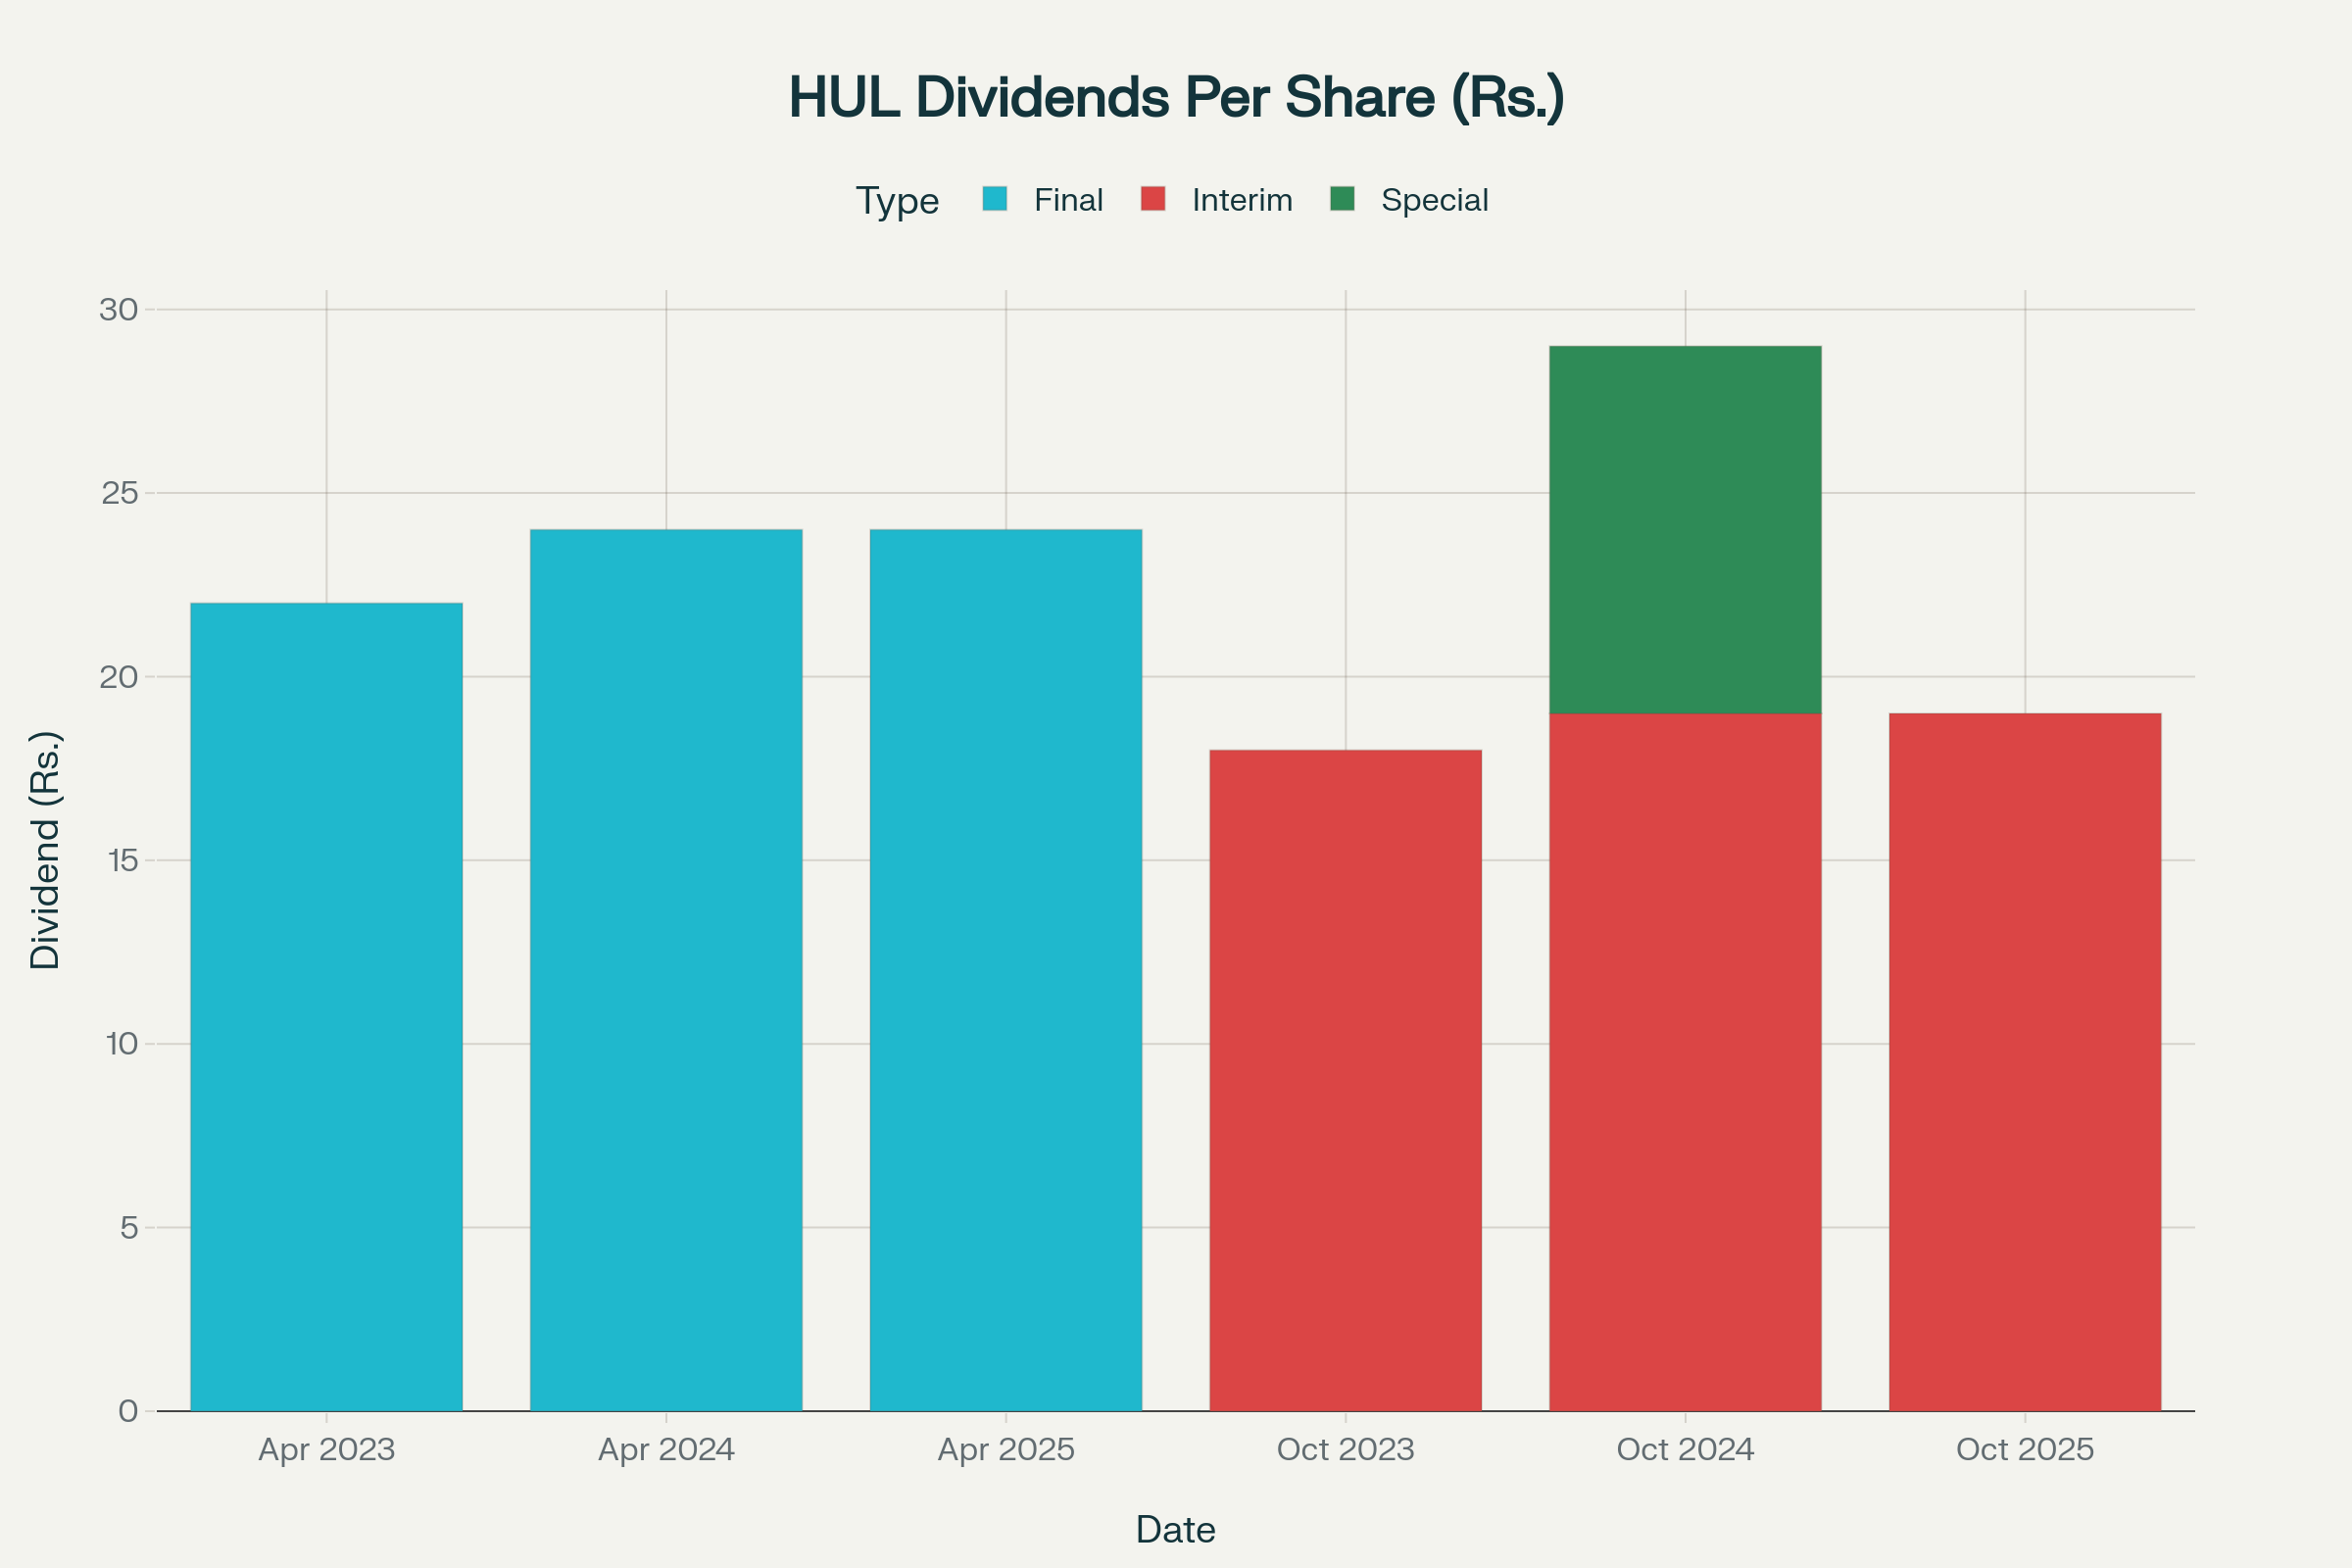
\includegraphics[width=\textwidth]{assets/Dividend_Payout_HUL.png}
        \caption{HUL Dividend Per Share (Rs.)}
    \end{minipage}
    \hfill
    \begin{minipage}{0.48\textwidth}
        \centering
        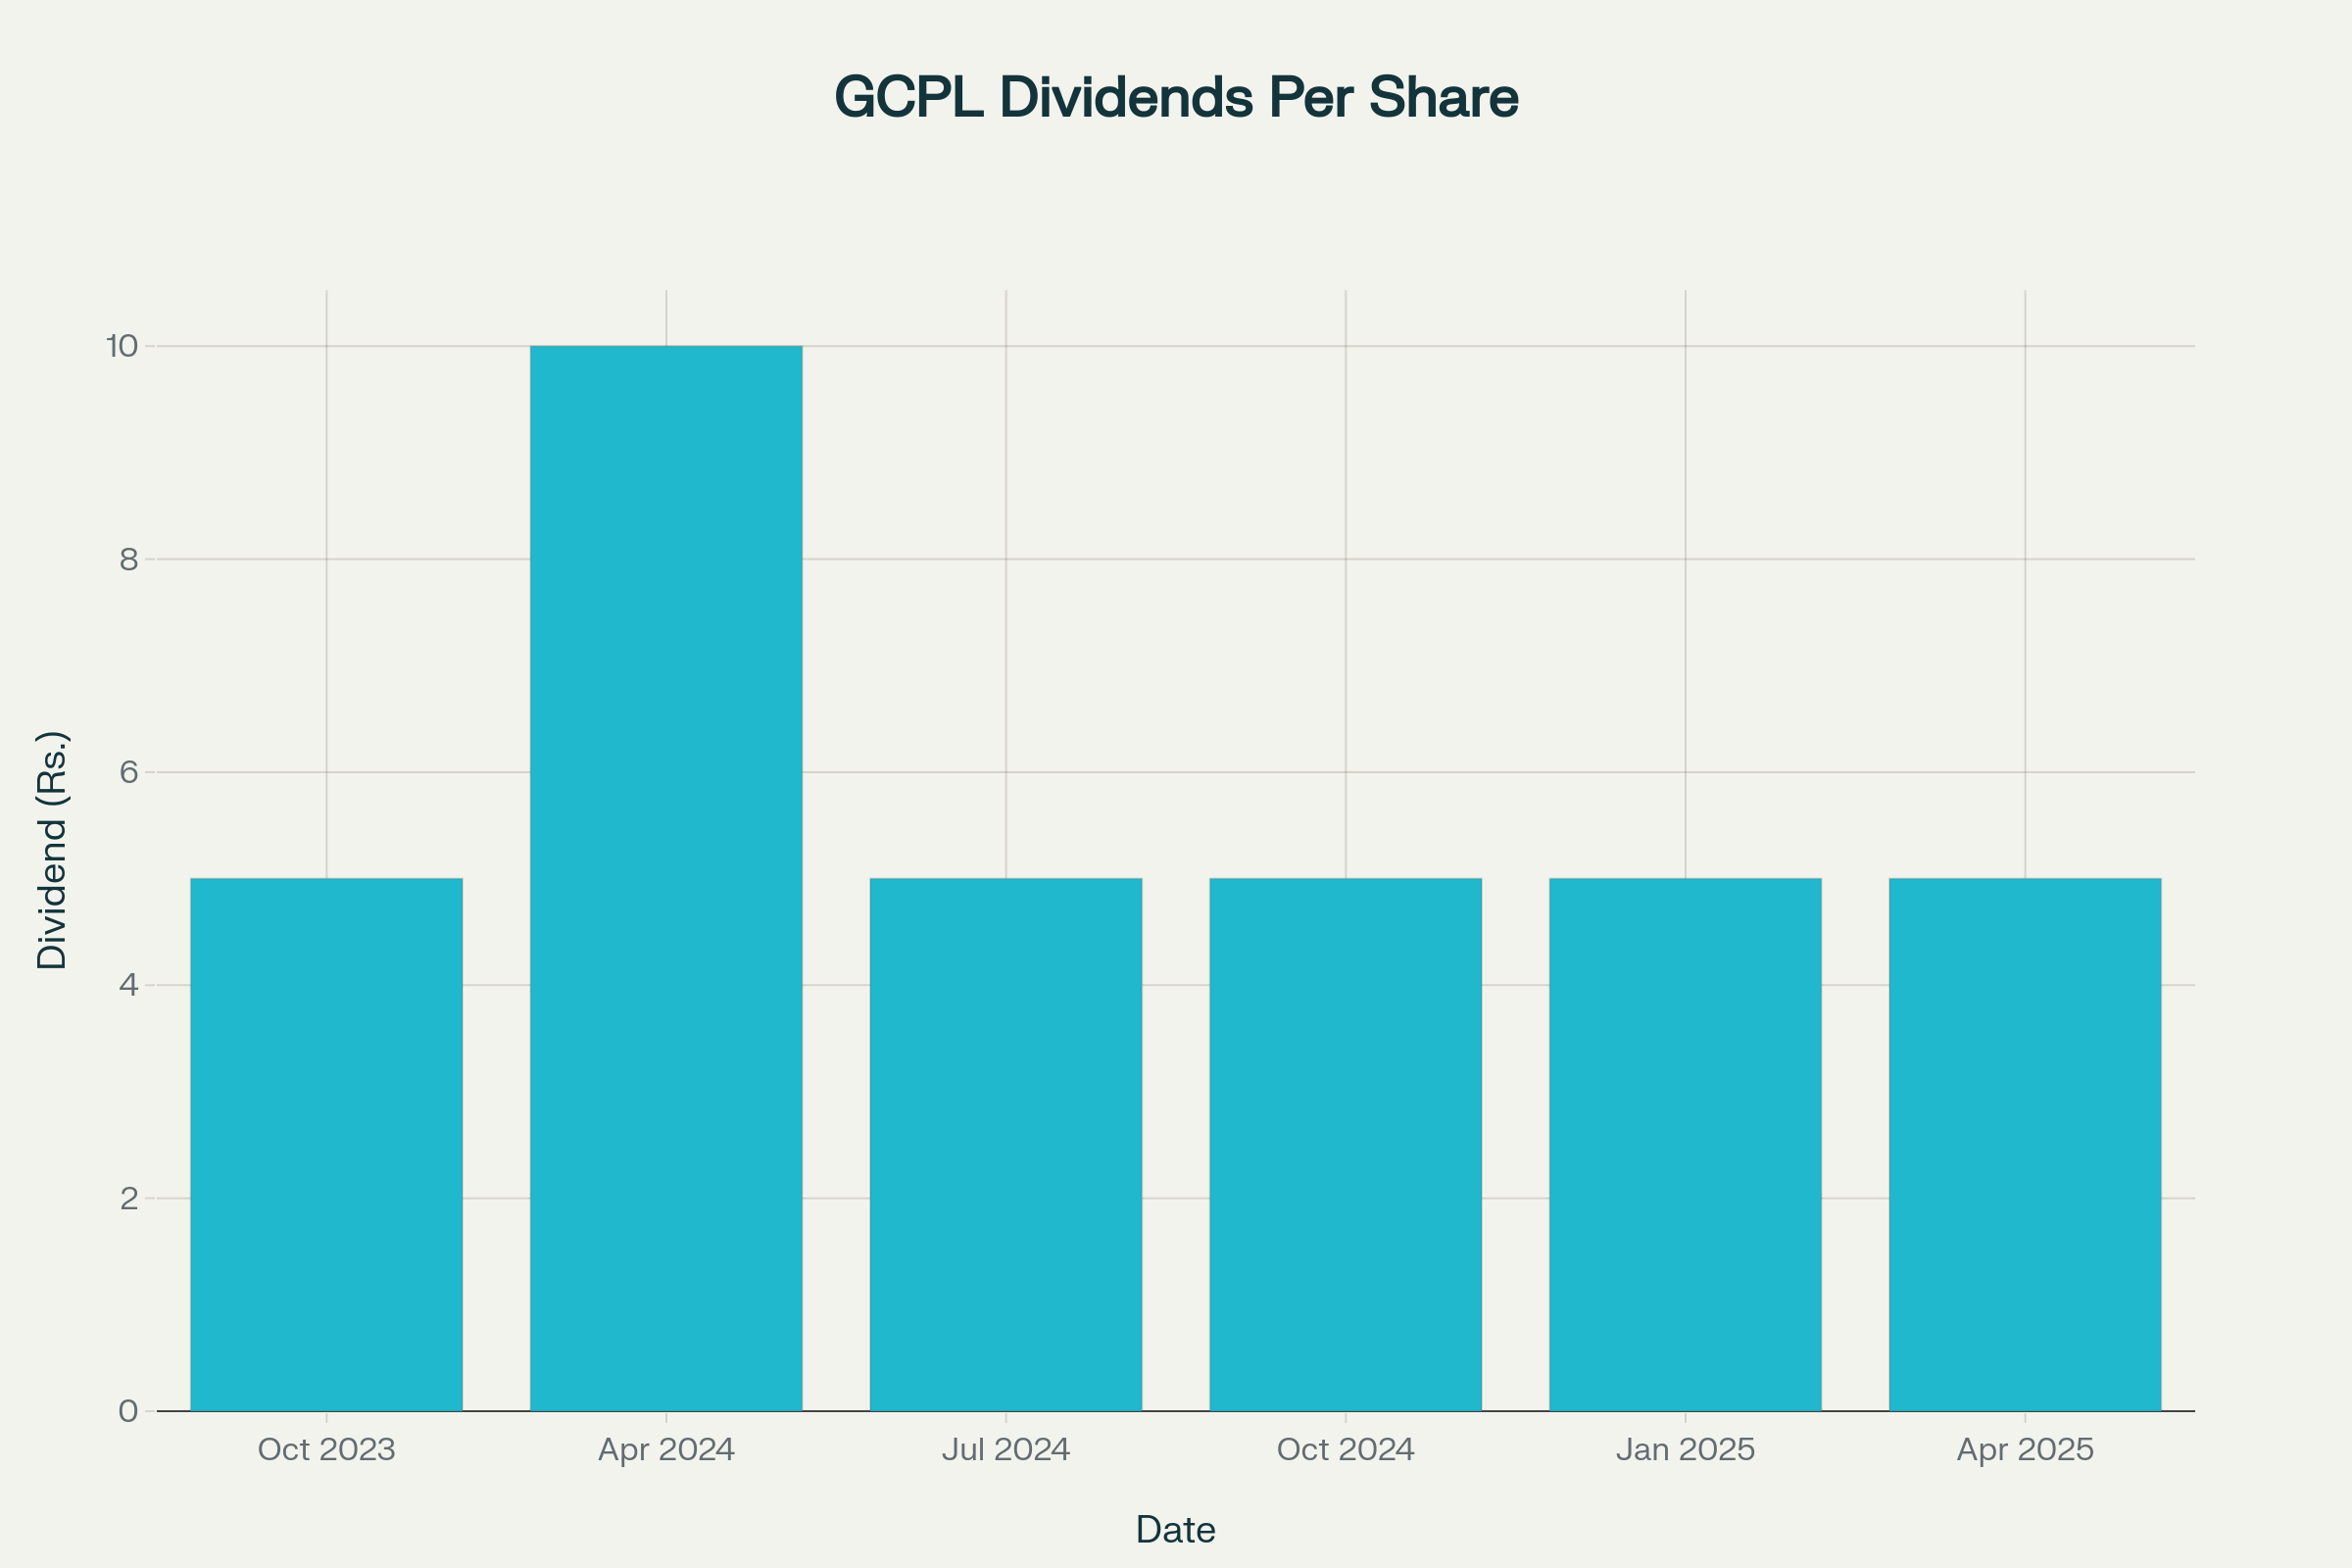
\includegraphics[width=\textwidth]{assets/Dividend_Payout_GCPL.png}
        \caption{GCPL Dividend Per Share (Rs.)}
    \end{minipage}
\end{figure}

\vspace{0.5cm}

\begin{figure}[H]
    \centering
    \begin{minipage}{0.48\textwidth}
        \centering
        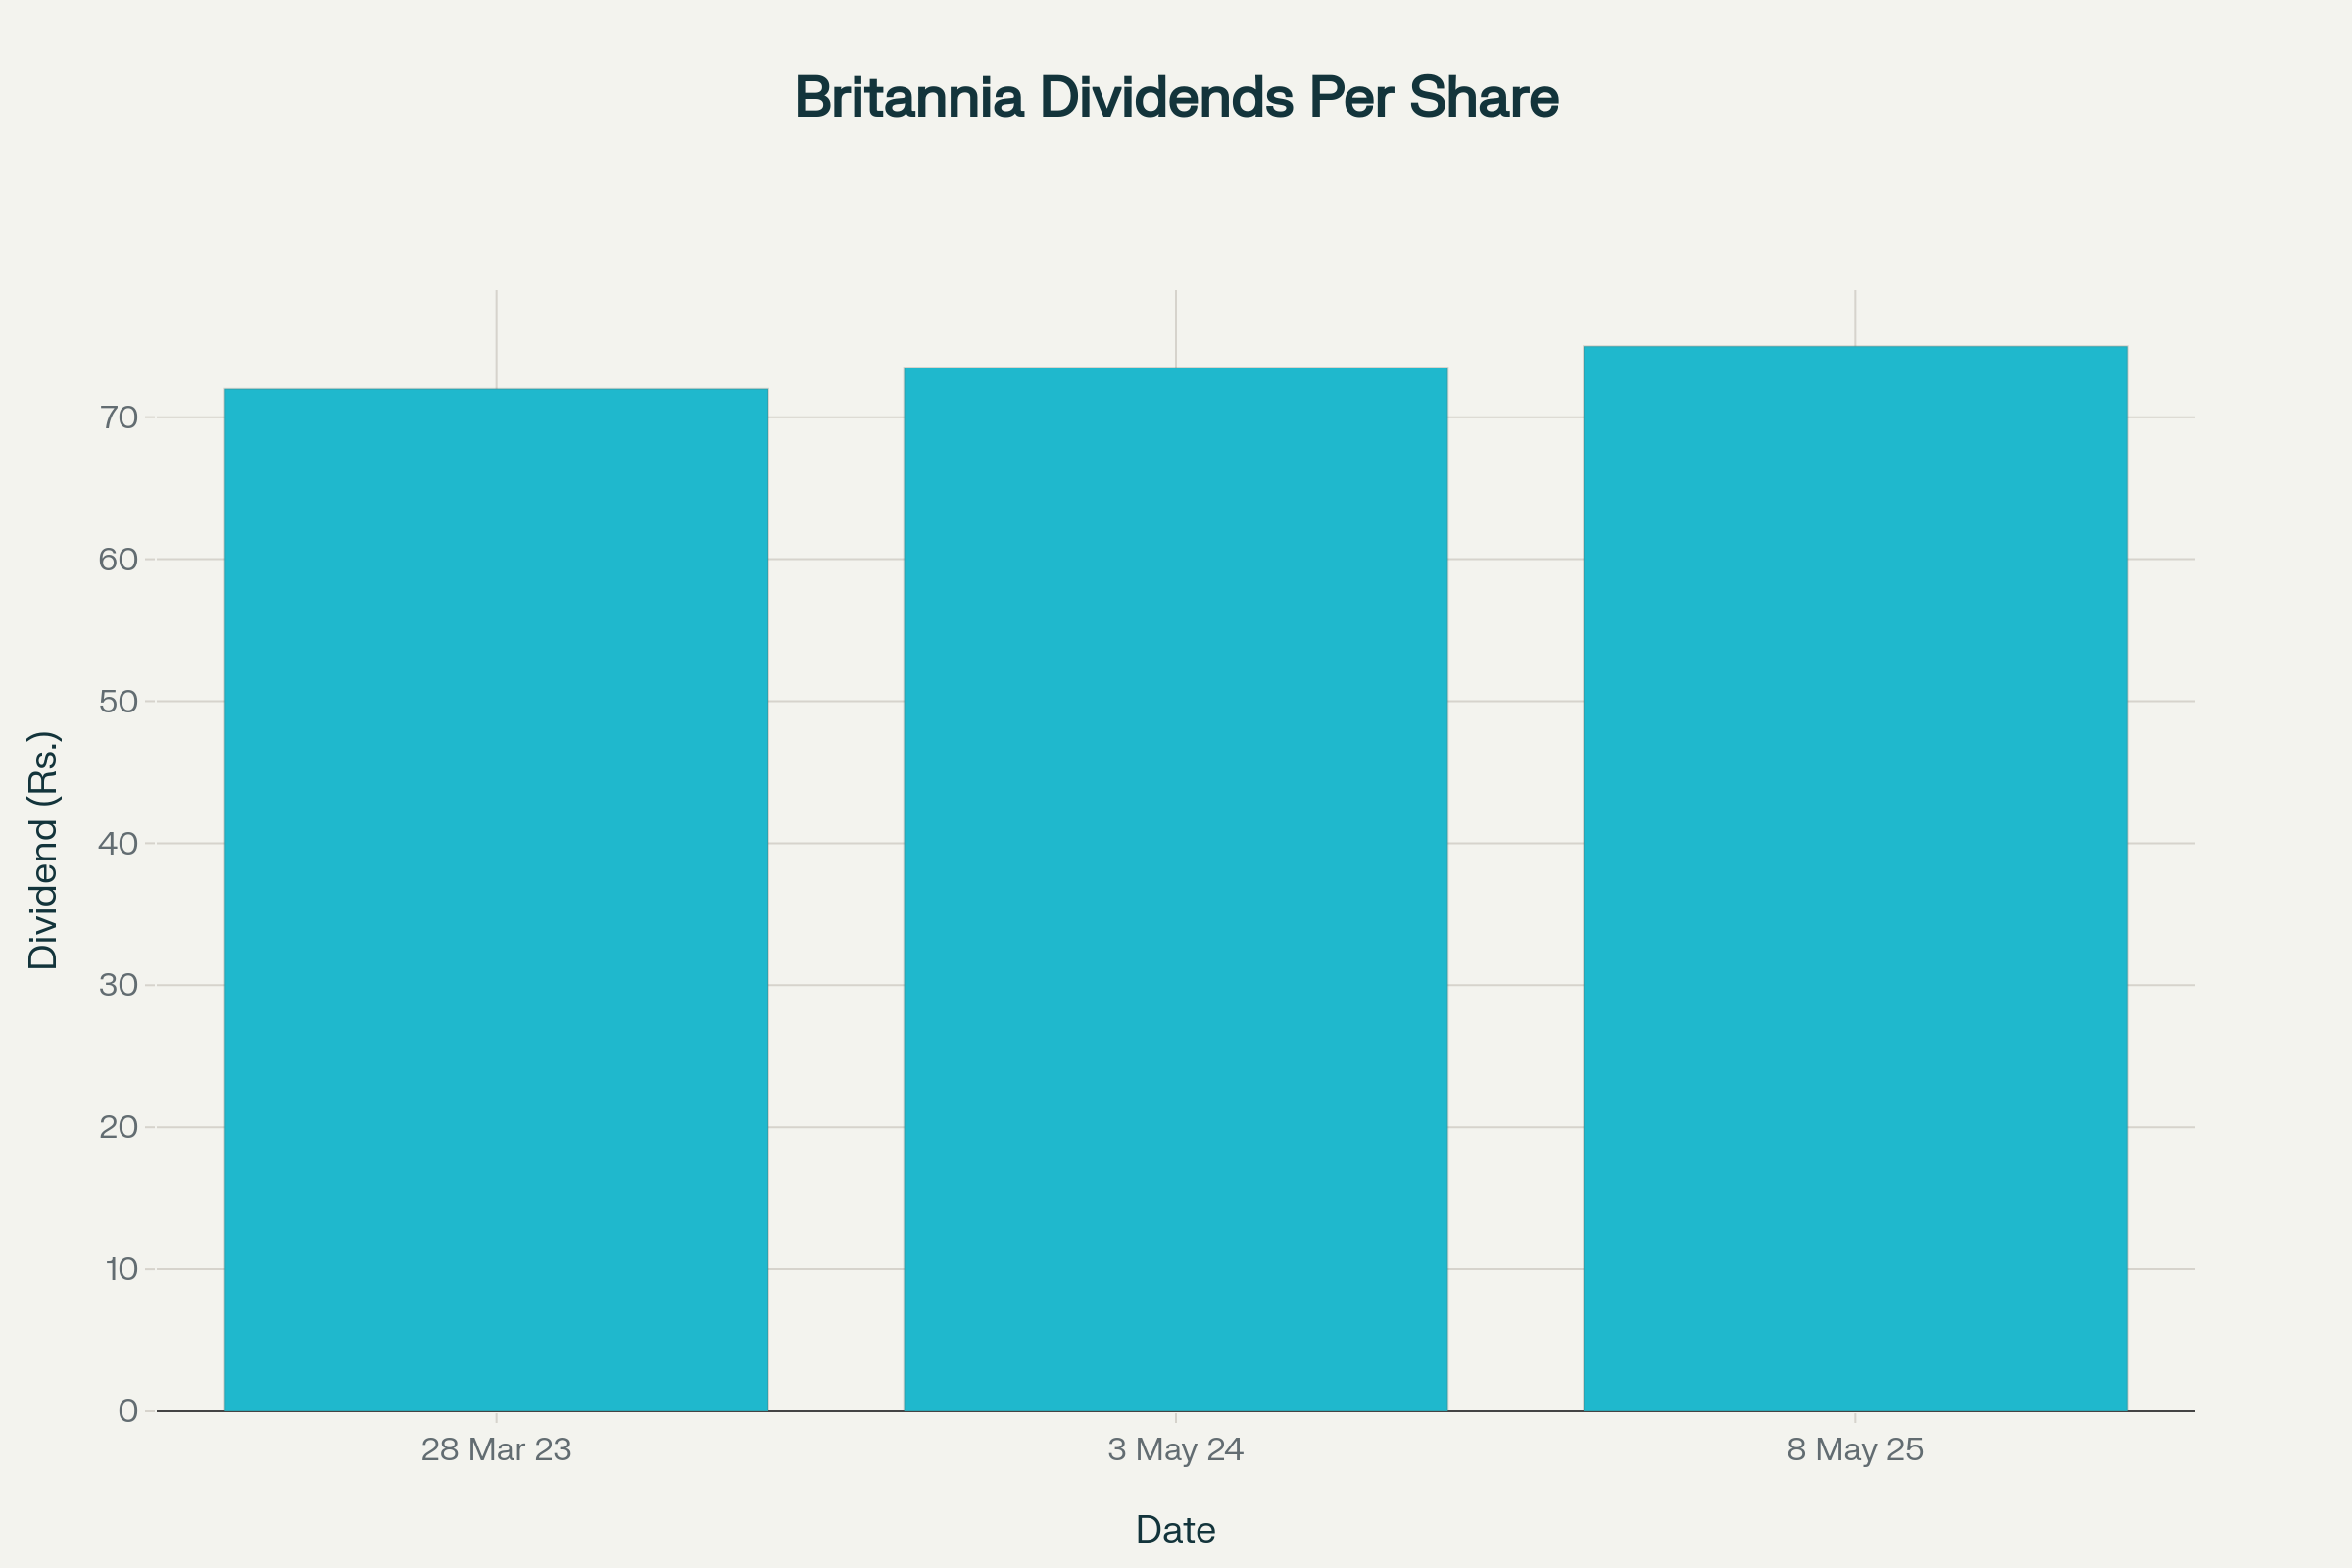
\includegraphics[width=\textwidth]{assets/Dividend_Payout_Britania.png}
        \caption{Britannia Dividend Per Share (Rs.)}
    \end{minipage}
    \hfill
    \begin{minipage}{0.48\textwidth}
        \centering
        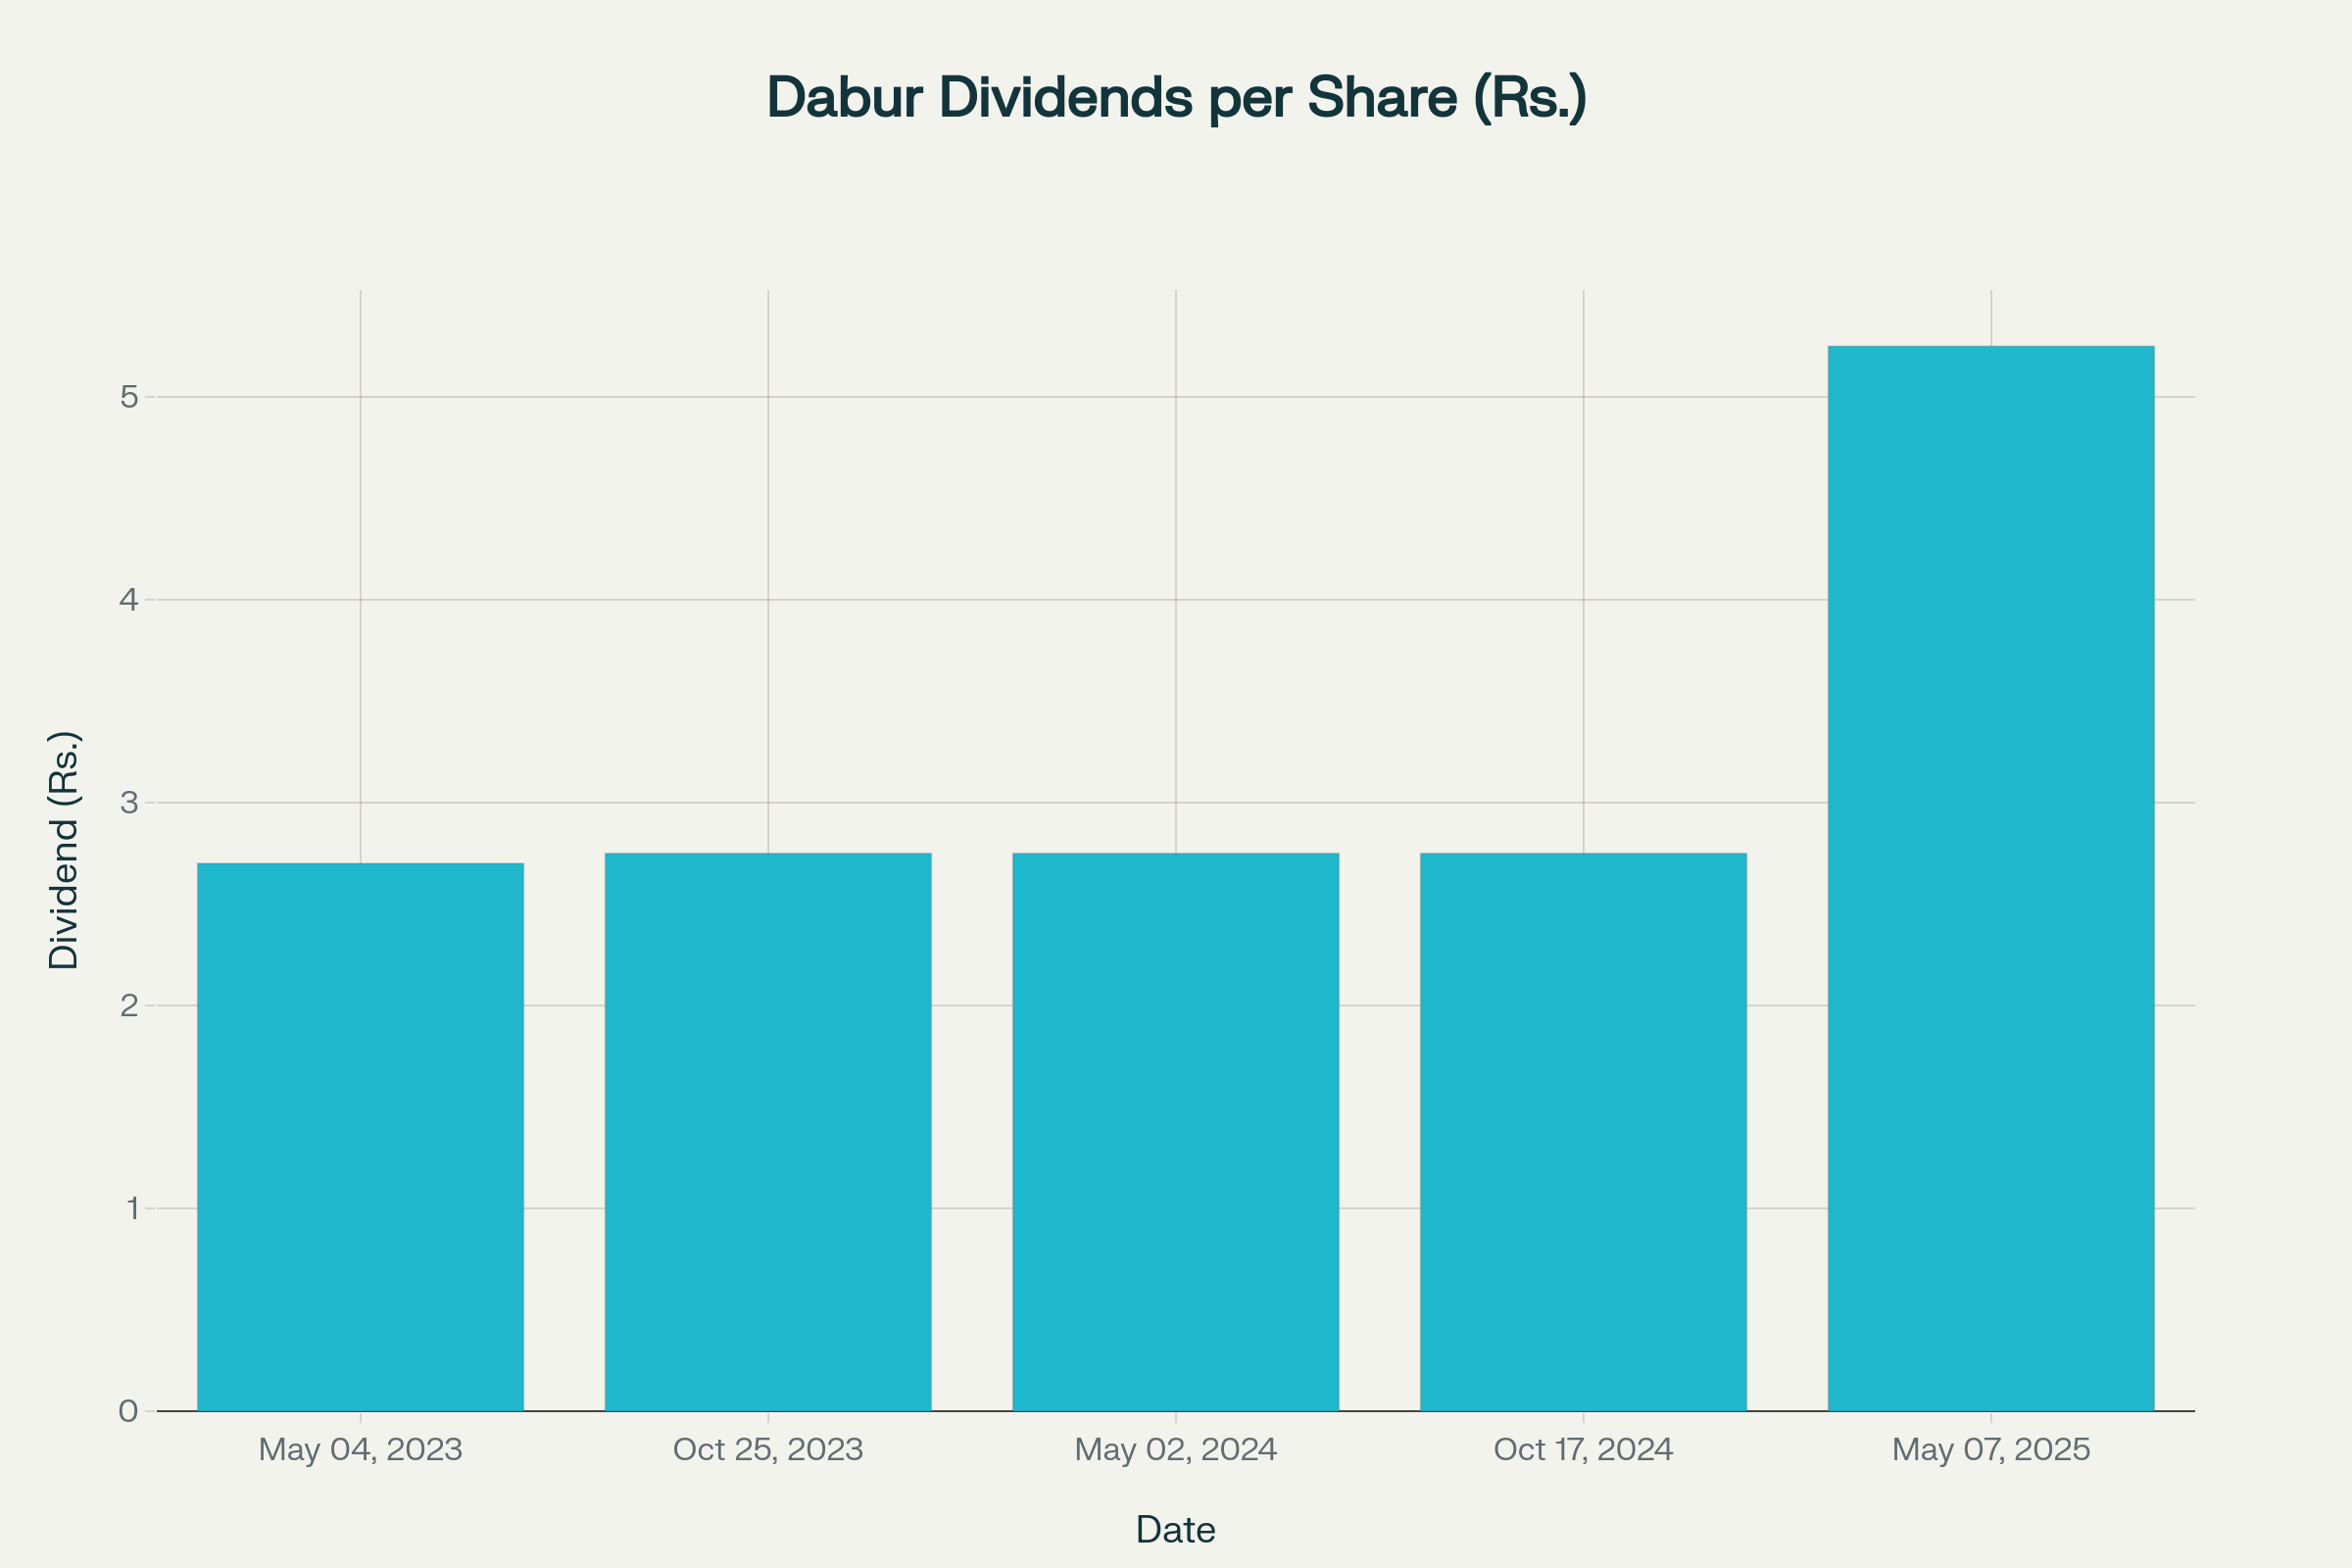
\includegraphics[width=\textwidth]{assets/Dividend_Payout_Dabur.png}
        \caption{Dabur Dividend Per Share (Rs.)}
    \end{minipage}
\end{figure}

\vspace{0.5cm}

\subsection*{Tata Consumer Products and ITC}

\begin{figure}[H]
    \centering
    \begin{minipage}{0.48\textwidth}
        \centering
        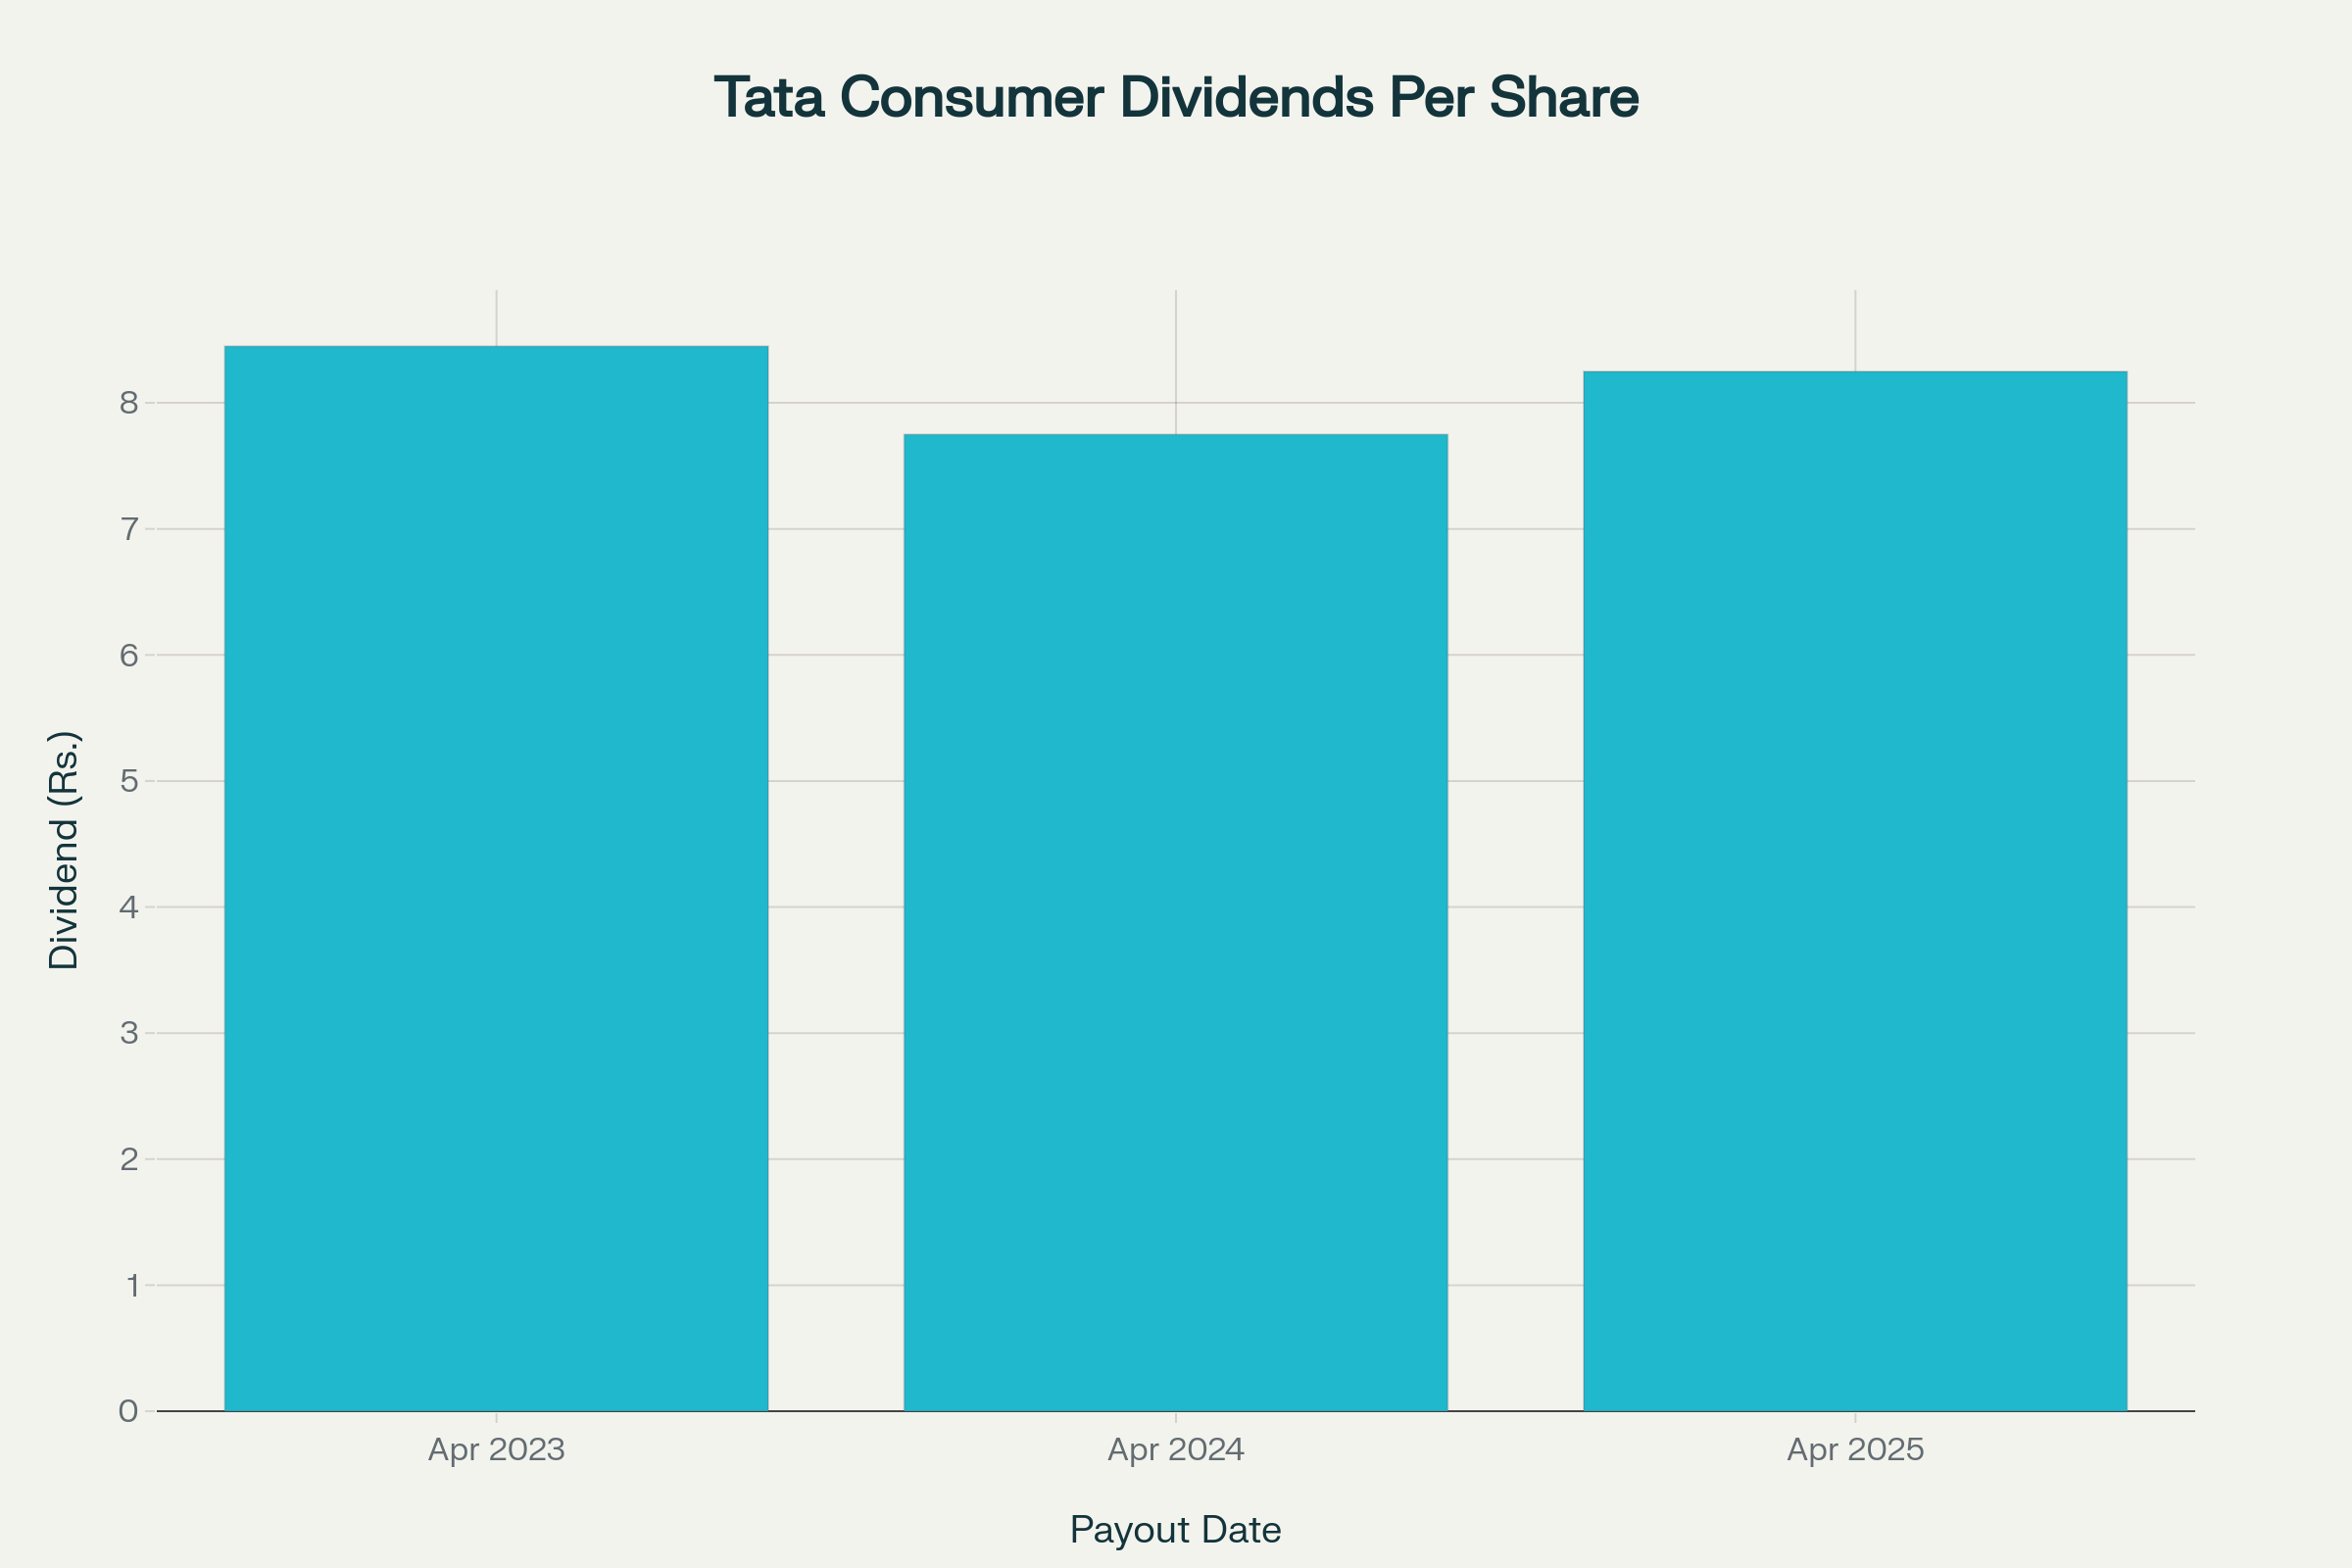
\includegraphics[width=\textwidth]{assets/Dividend_Payout_Tata.png}
        \caption{Tata Consumer Products Dividend Per Share (Rs.)}
    \end{minipage}
    \hfill
    \begin{minipage}{0.48\textwidth}
        \centering
        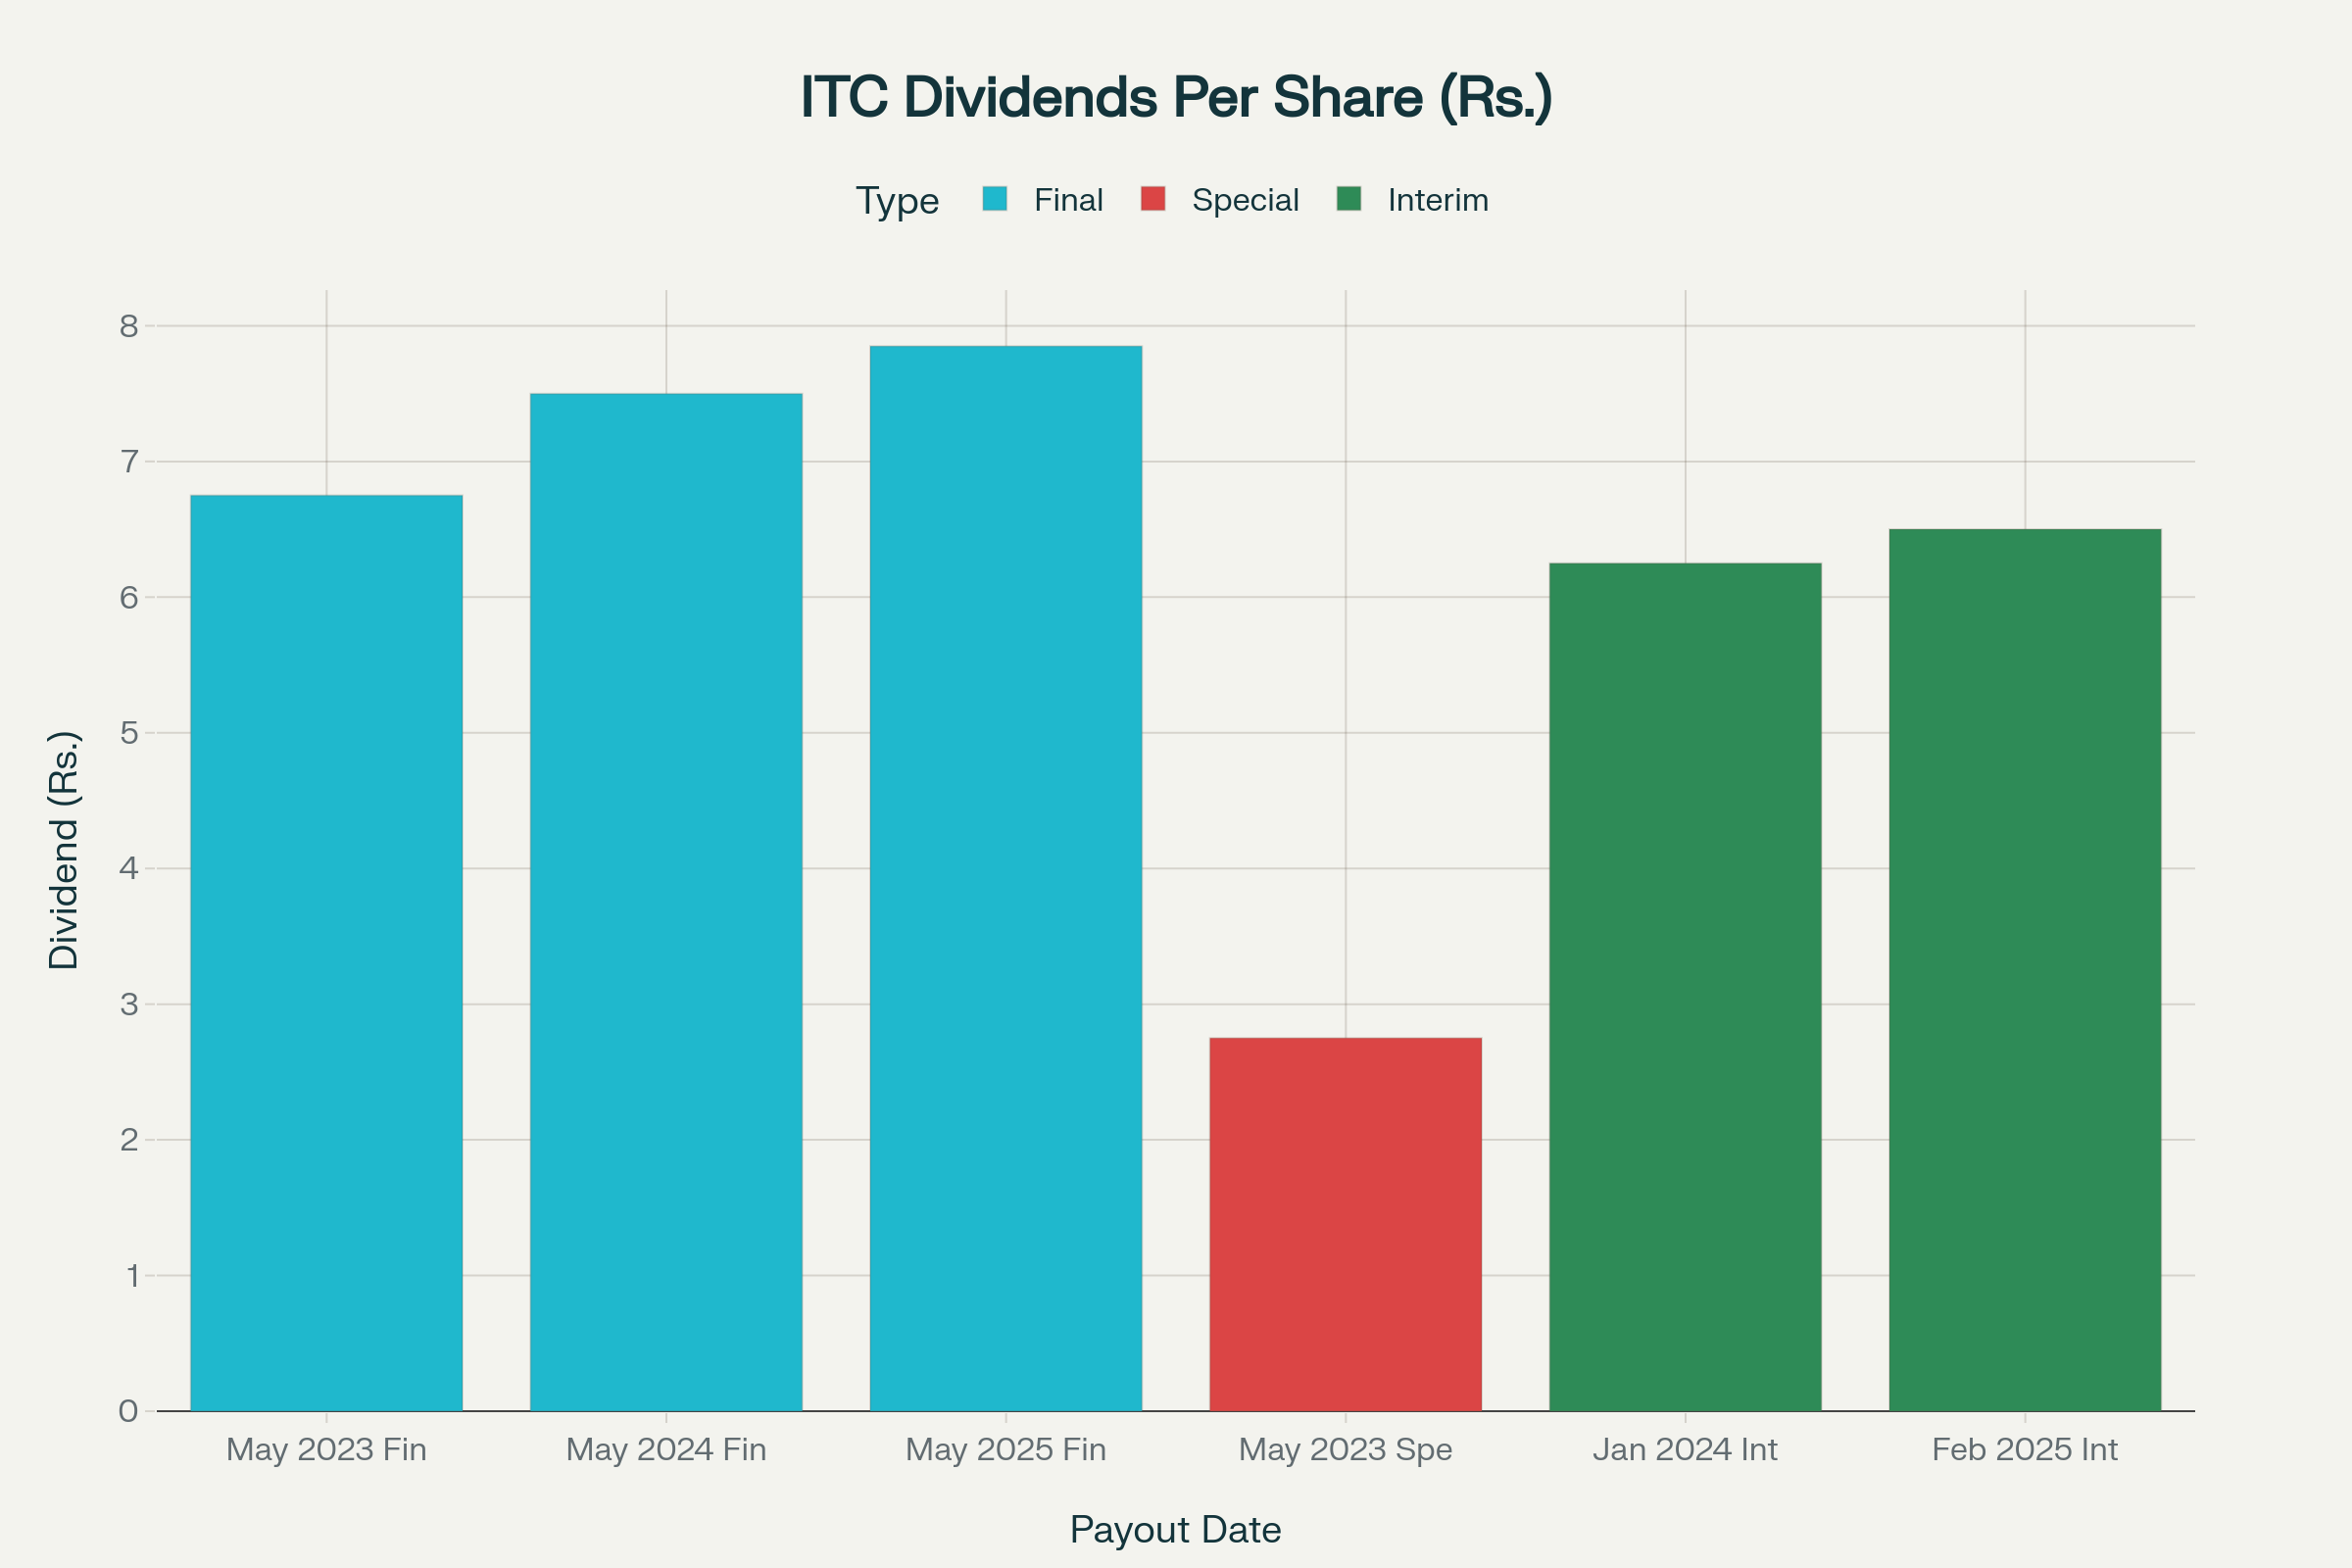
\includegraphics[width=\textwidth]{assets/Dividend_Payout_ITC.png}
        \caption{ITC Dividend Per Share (Rs.)}
    \end{minipage}
\end{figure}

% ===============================================
% APPENDIX: NOTES
% ===============================================
\newpage
\appendix
\chapter{Notes and References}

\begin{itemize}
    \item \textbf{NIC Code:} Represents the National Industrial Classification code. The specific codes have been gathered and contextualized for each major business activity.
    
    \item \textbf{CEO/Chairman:} Names and tenures are up-to-date as of October 2025.
    
    \item \textbf{Dividends:} All graphs show per-share dividend values issued in the last two years for each company (Final, Interim, Special).
\end{itemize}

\end{document}
